\thispagestyle{timhieukhoahocnone}
\pagestyle{timhieukhoahoc}
\everymath{\color{timhieukhoahoc}}
\blfootnote{$^1$\text{\color{timhieukhoahoc}https://phys.org/news/2023-10-scientists-nobel-prize-physics-electrons.html}}
\blfootnote{$^2$\text{\color{timhieukhoahoc}Viện Toán học.}}

\graphicspath{{../timhieukhoahoc/pic/}}
\begingroup
\AddToShipoutPicture*{\put(0,616){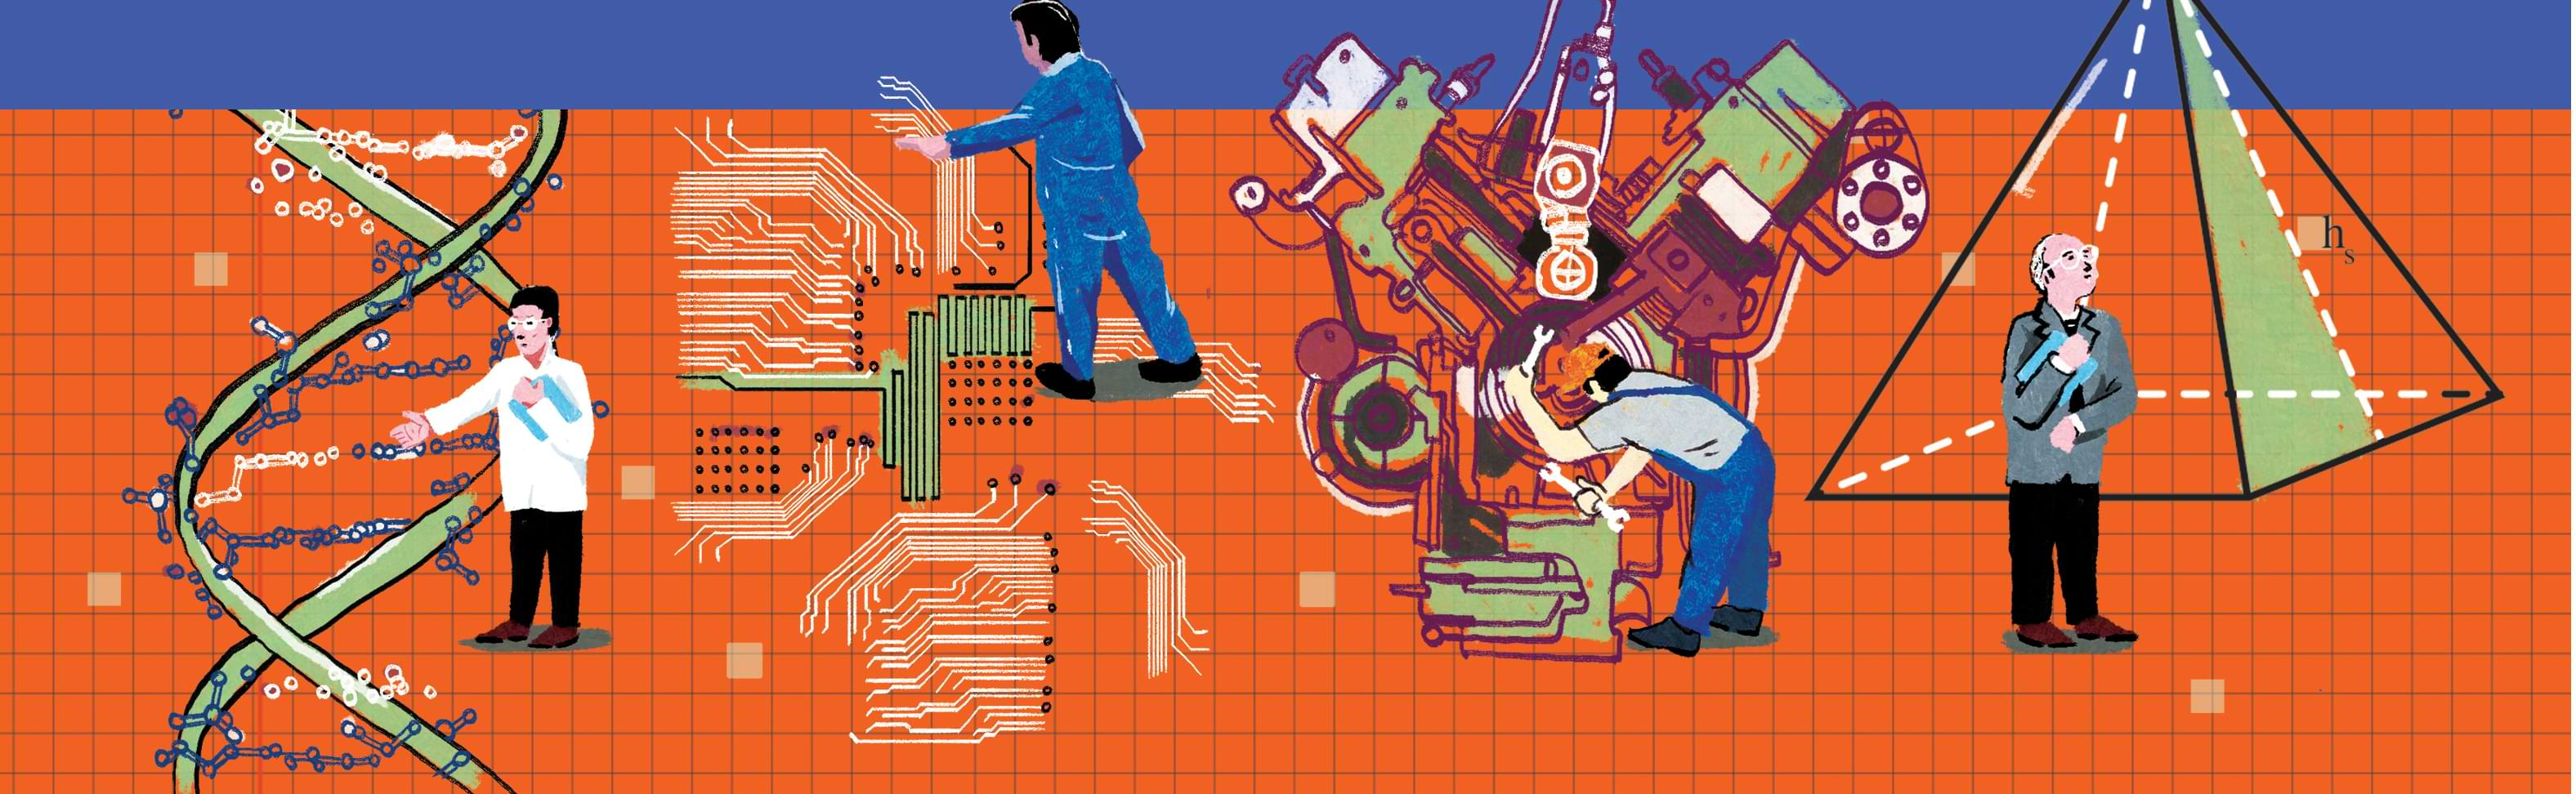
\includegraphics[width=19.3cm]{../bannertimhieu}}}
\AddToShipoutPicture*{\put(60,533){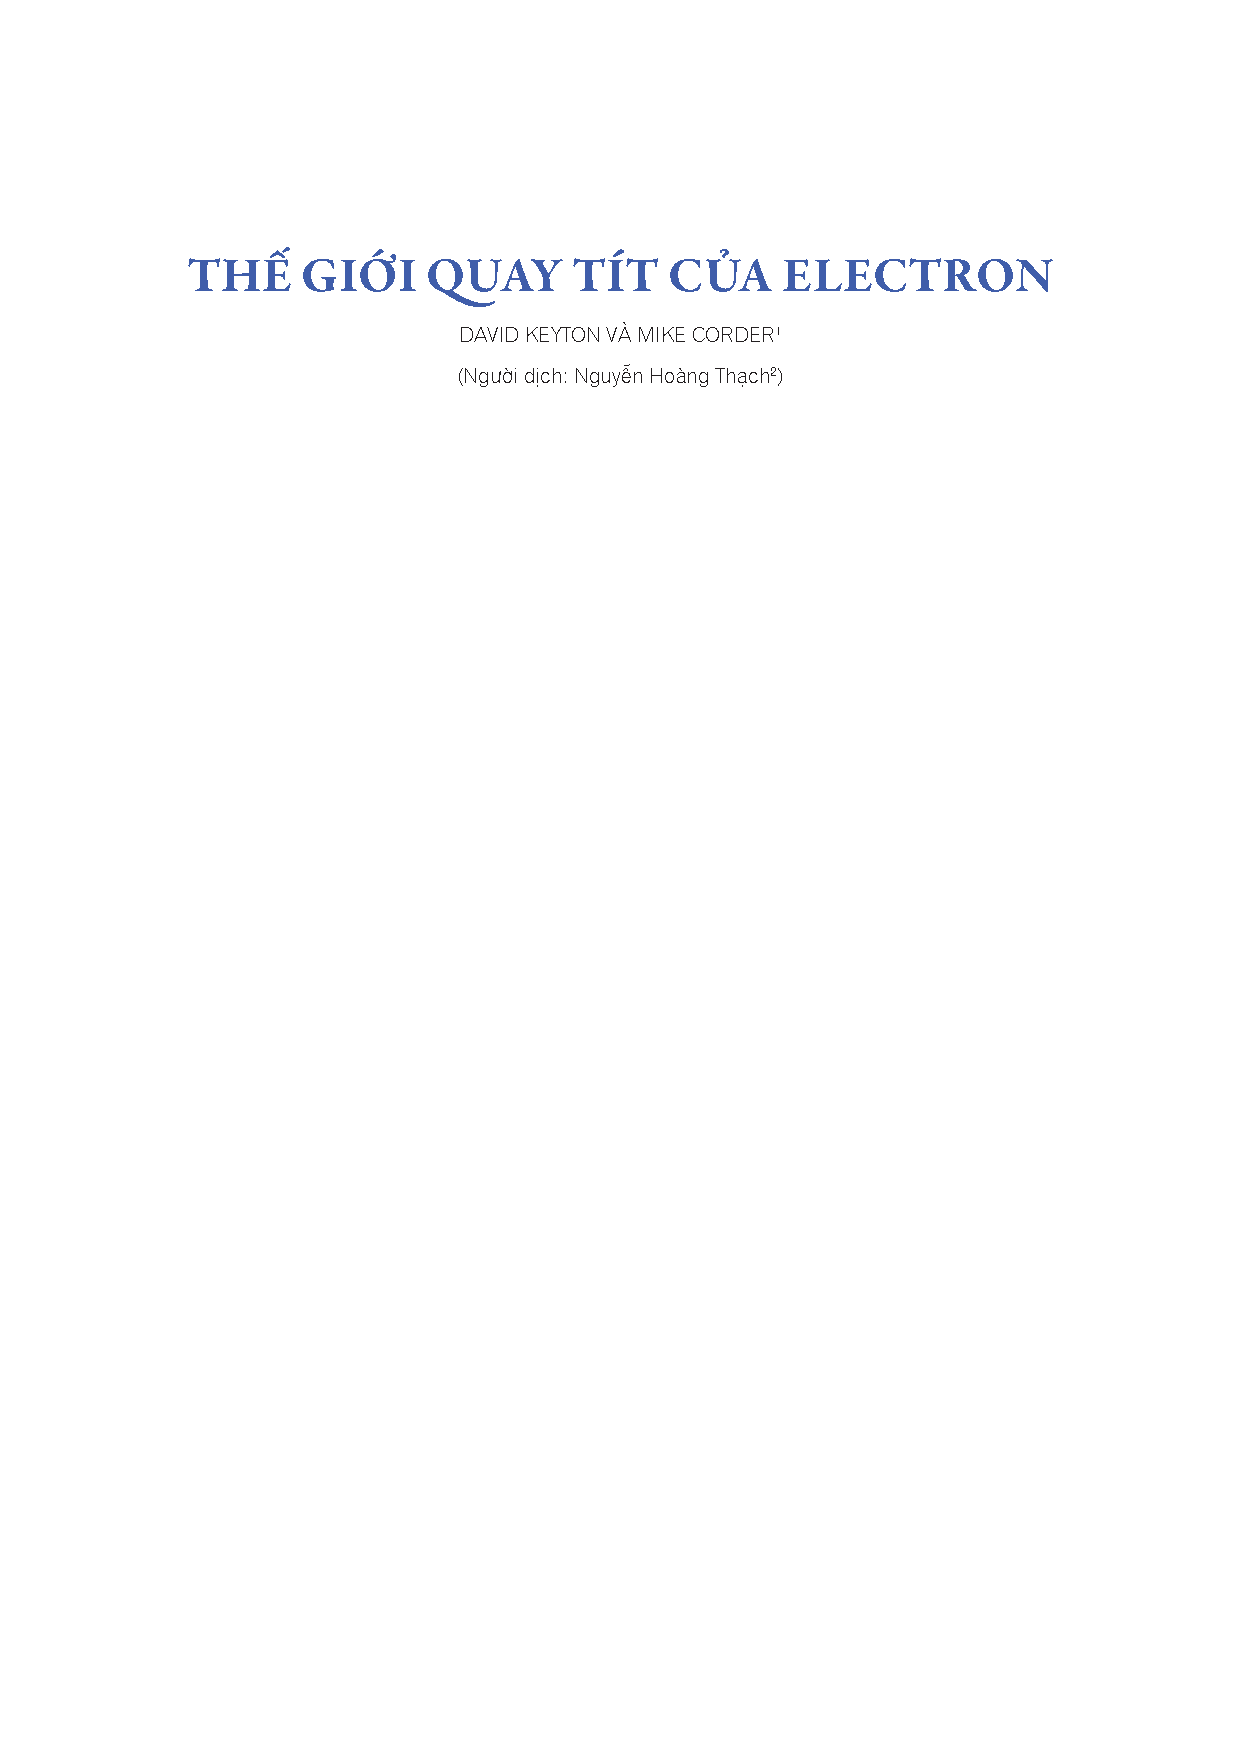
\includegraphics[scale=1]{../tieude.pdf}}}
\centering
\endgroup
\vspace*{170pt}

\begin{multicols}{2}
	Hôm thứ ba ngày $3$ tháng $10$ vừa qua, ba nhà khoa học đã giành được Giải Nobel Vật lý $2023$ nhờ mang đến cho chúng ta cái nhìn đầu tiên về thế giới siêu tốc độ của các electron quay tít, một lĩnh vực có thể sẽ giúp cải tiến các thiết bị điện tử hoặc chẩn đoán bệnh.
	\begin{figure}[H]
		\vspace*{-5pt}
		\centering
		\captionsetup{labelformat= empty, justification=centering}
		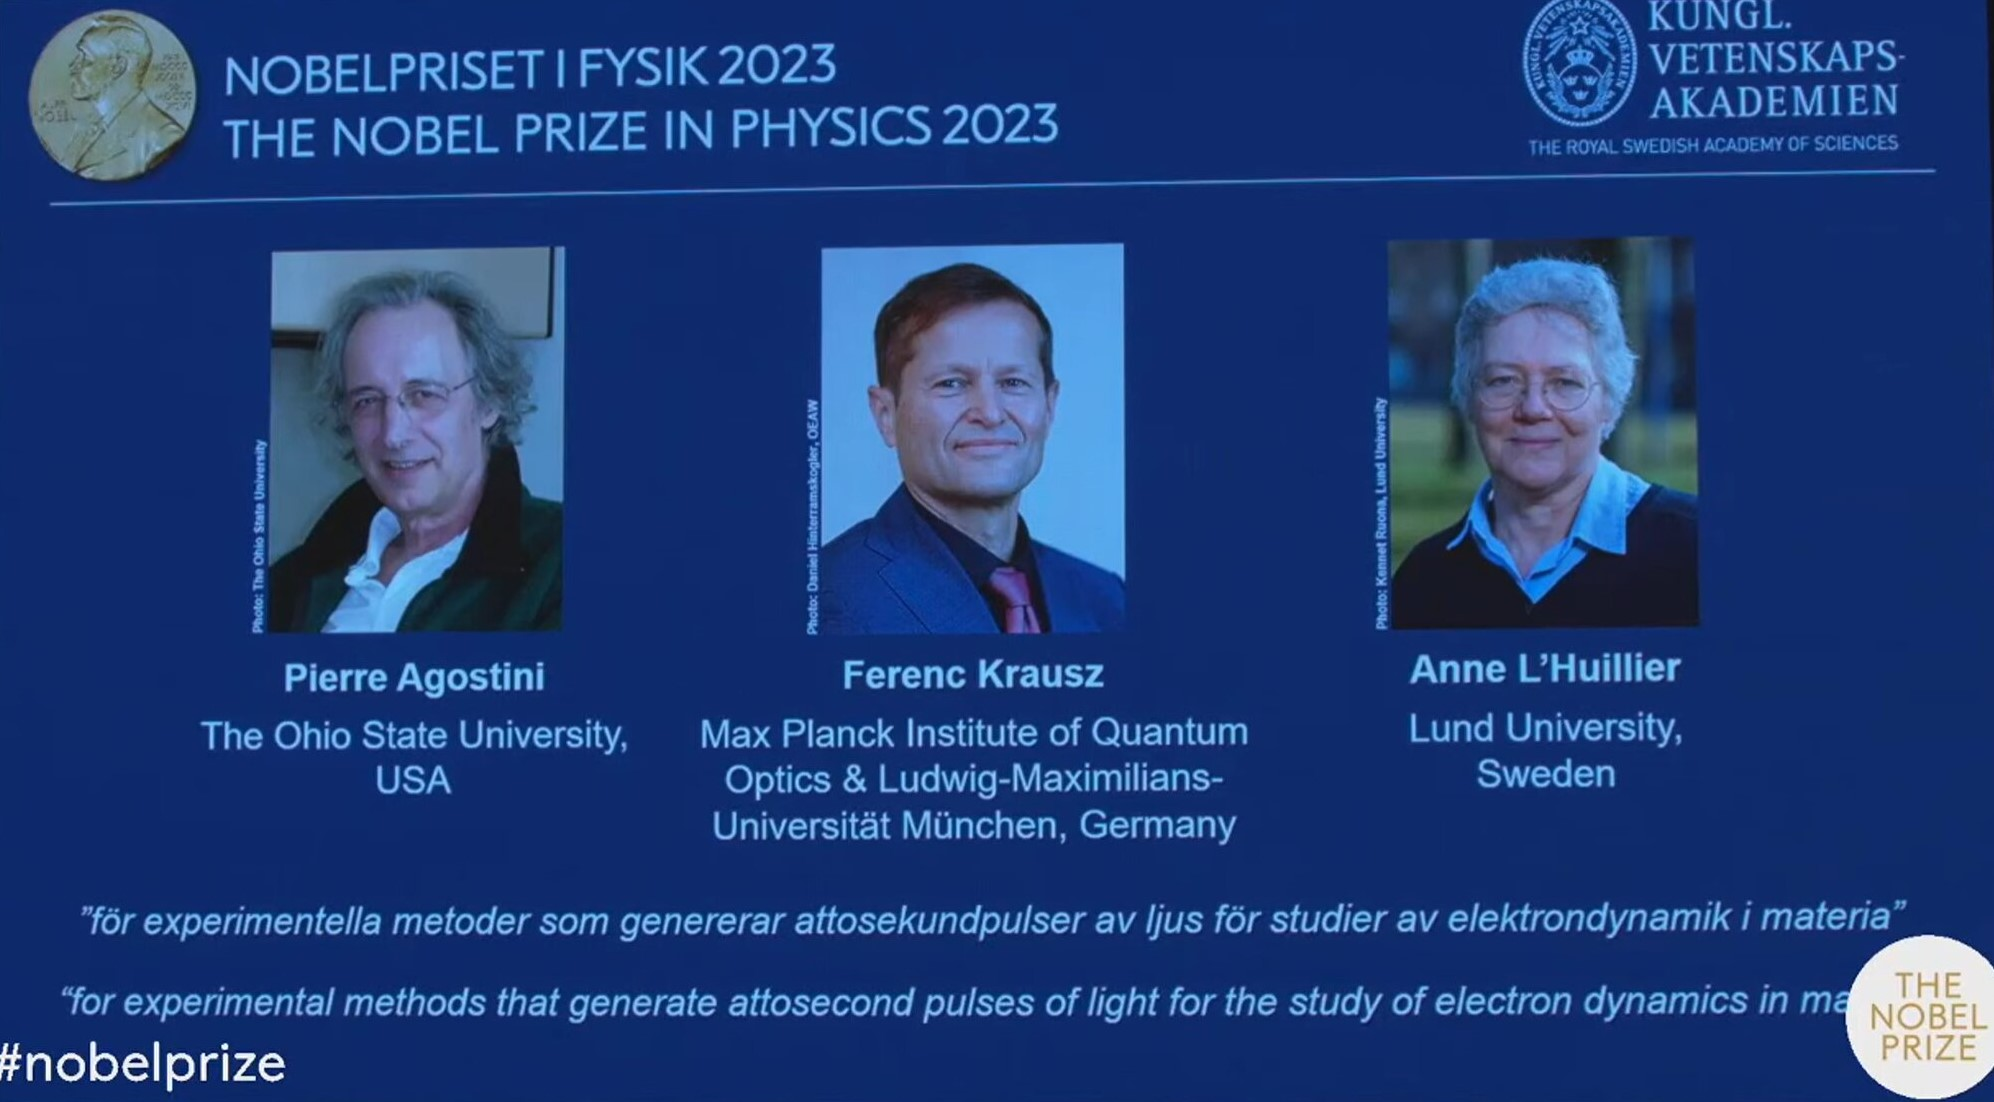
\includegraphics[width= 1\linewidth]{1}
		\caption{\small\textit{\color{timhieukhoahoc}Ảnh: Viện Hàn lâm Khoa học Hoàng gia Thụy~Điển.}}
		\vspace*{-10pt}
	\end{figure}
	Giải thưởng được trao cho nhà vật lý Pháp -- Thụy Điển Anne L'Huillier, nhà vật lý người Pháp Pierre Agostini và nhà vật lý gốc Hungary Ferenc Krausz, vì công trình của họ về thành phần tí hon chạy quanh hạt nhân của nguyên tử và là cái cơ bản của hầu như mọi thứ: hóa học, vật lý, cơ thể và vật dụng của chúng ta.
	\vskip 0.1cm
	Theo các chuyên gia, electron di chuyển nhanh đến nỗi con người không thể cô lập được chúng, nhưng bằng cách quan sát trong những tích tắc nhỏ nhất có thể, các nhà khoa học hiện đã có cái nhìn thoáng qua ``mờ mờ" về chúng, qua đó mở ra nhiều ngành khoa học hoàn toàn mới.
	\vskip 0.1cm
	``Electron di chuyển rất nhanh, và chúng thực sự là lực lượng lao động ở mọi nơi," Mats Larsson, thành viên Ủy ban Giải thưởng Nobel, cho biết. ``Một khi có thể điều khiển và hiểu được electron, bạn đã tiến được một bước lớn."
	\vskip 0.1cm
	L'Huillier, giáo sư tại Đại học Lund, Thụy Điển, là người phụ nữ thứ năm được Nobel Vật lý.
	\vskip 0.1cm
	``Gửi đến tất cả phụ nữ, tôi muốn nói rằng nếu bạn thích, nếu bạn có một chút đam mê với những thách thức kiểu này, hãy theo đuổi nó," bà nói với hãng tin AP.
	\vskip 0.1cm
	\textbf{\color{timhieukhoahoc}Khám phá được trao Giải Nobel Vật lý}
	\vskip 0.1cm
	Ba nhà khoa học, độc lập với nhau, đã sử dụng xung laser ngày càng nhanh để bắt lại hoạt động của nguyên tử xảy ra ở tốc độ chóng mặt -- một phần tỷ tỷ giây, hay một \textit{atto} giây\footnote[3]{\color{timhieukhoahoc}$1$ atto giây = $10^{-18}$ giây -- Pi.} -- giống như cách các nhiếp ảnh gia sửa dụng cửa trập tốc độ cao để chụp ảnh chim ruồi đang hút mật hoa.
	\begin{figure}[H]
		\vspace*{5pt}
		\centering
		\captionsetup{labelformat= empty, justification=centering}
		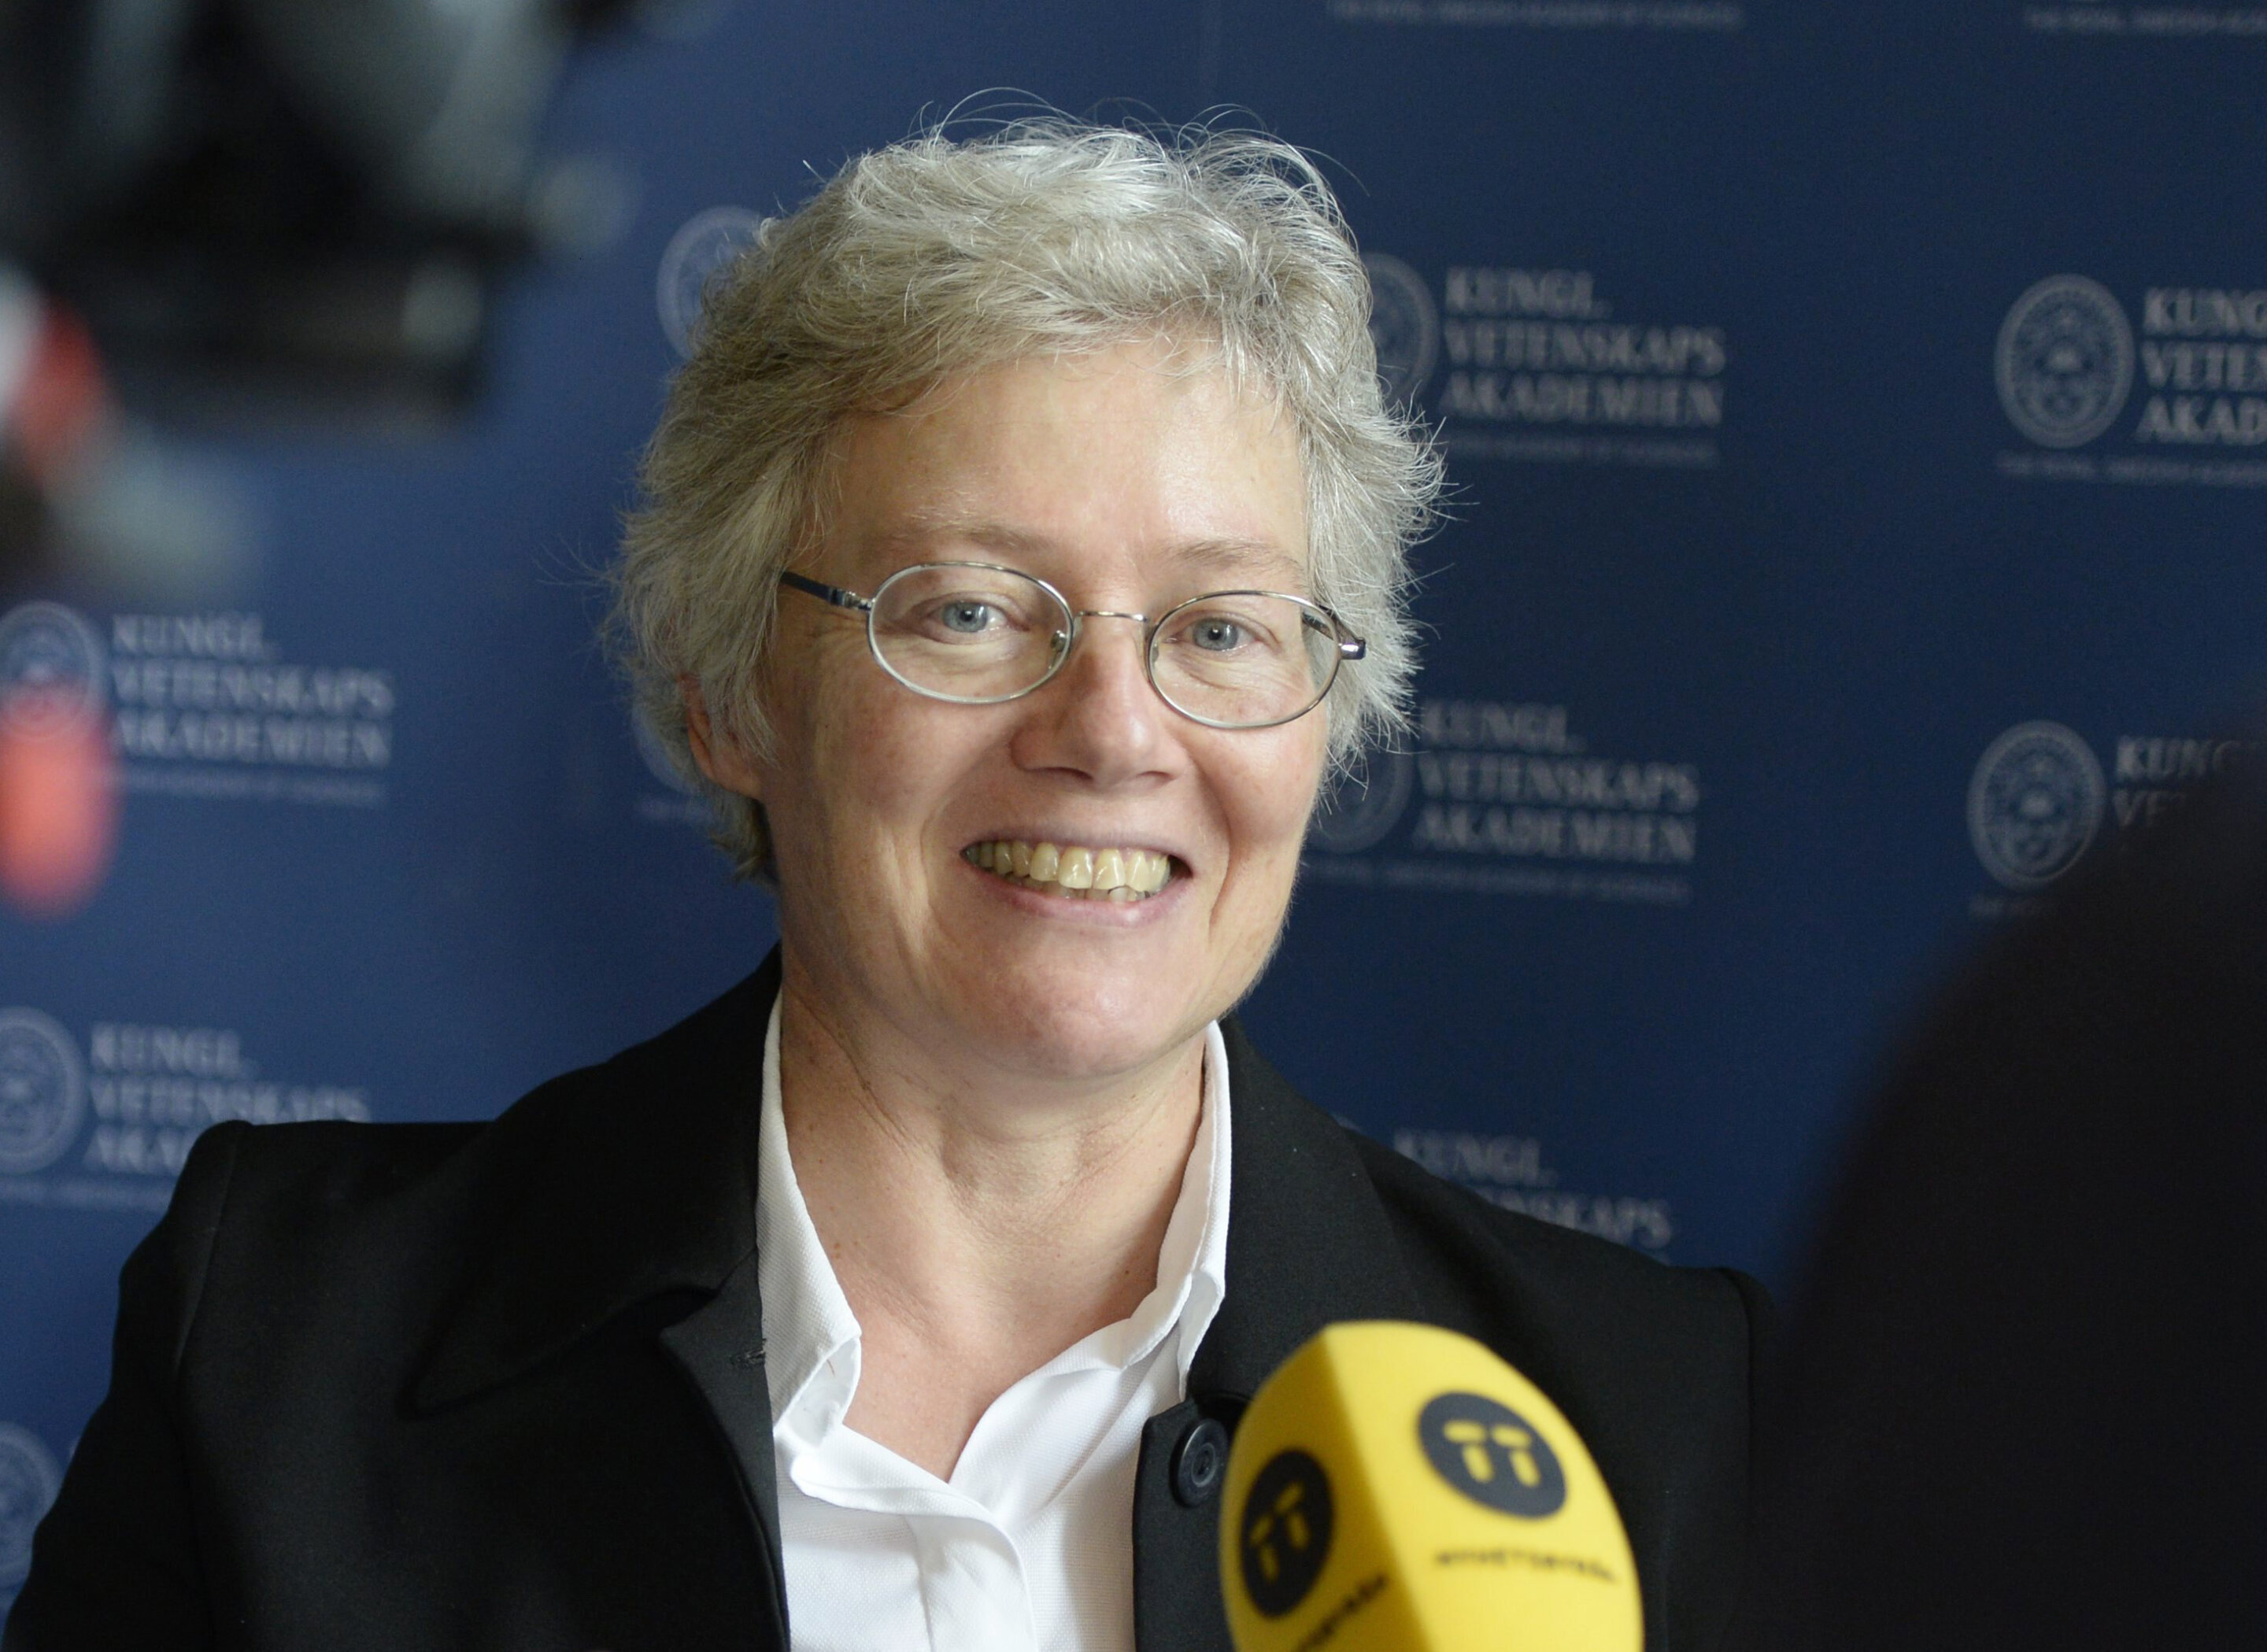
\includegraphics[width= 1\linewidth]{3}
		\caption{\small\textit{\color{timhieukhoahoc}Nhà vật lý Pháp--Thụy Điển Anne L'Huillier}}
		\vspace*{-10pt}
	\end{figure}
	Khoảng thời gian đó ngắn đến mức nào?
	\vskip 0.1cm
	``Hãy lấy một giây, là khoảng thời gian của một nhịp tim," chủ tịch Ủy ban Giải thưởng Nobel, Eva Olsson nói. Để đạt đến cỡ atto giây, cần chia nó cho $1000$ sáu lần.
	\vskip 0.1cm
	Nhà vật lý Mark Pearce, thành viên Ủy ban Giải thưởng Nobel, nói rằng ``số atto giây trong một giây bằng số giây đã trôi qua kể từ Big Bang, khoảng $13{,}8$ tỷ năm trước."
	\vskip 0.1cm
	Nhưng ngay cả khi ``thấy" được electron, các nhà khoa học cũng không thấy được hết.
	\vskip 0.1cm
	``Bạn có thể thấy nó ở phía bên này hay phía bên kia của một phân tử," L'Huillier, năm nay $65$ tuổi, nói. ``Nó vẫn rất mờ."
	\vskip 0.1cm
	``Electron giống sóng, như sóng trên mặt nước, nhiều hơn là giống hạt, và cái chúng tôi đo với kỹ thuật của mình là vị trí của ngọn sóng," bà nói thêm.
	\vskip 0.1cm
	\textbf{\color{timhieukhoahoc}Vì sao electron quan trọng?}
	\vskip 0.1cm
	Electron có vai trò then chốt vì chúng chính là ``cách các nguyên tử liên kết với nhau," L'Huillier nói. Đó là nơi diễn ra các phản ứng hóa học.
	\vskip 0.1cm
	``Dù ta không thể thấy chúng, electron hiện diện khắp mọi nơi trong cuộc sống của chúng ta, theo cả nghĩa cuộc sống sinh học lẫn cuộc sống kỹ thuật, cuộc sống hàng ngày," Krausz nói tại một buổi họp báo. ``Trong cuộc sống sinh học, electron tạo nên chất keo giữa các nguyên tử, từ đó các nguyên tử tạo thành phân tử, và các phân tử này là những viên gạch nhỏ nhất để xây dựng nên mọi cơ thể sống."
	\vskip 0.1cm
	Và nếu muốn hiểu cách chúng làm việc, bạn cần biết cách chúng di chuyển, Krausz nói.
	\vskip 0.1cm
	Hiện tại, khoa học này phục vụ cho việc tìm hiểu vũ trụ của chúng ta, nhưng người ta hy vọng nó cuối cùng sẽ có ứng dụng thực tế trong điện tử, chẩn đoán bệnh và hóa học cơ bản.
	\vskip 0.1cm
	L'Huillier nói rằng công trình của bà cho thấy tầm quan trọng của việc tiến hành nghiên cứu cơ bản mà không cần biết có ứng dụng trong tương lai hay không: bà đã làm việc với nó $30$ năm trước khi những ứng dụng thực tế trở nên rõ ràng hơn.
	\begin{figure}[H]
		\vspace*{-5pt}
		\centering
		\captionsetup{labelformat= empty, justification=centering}
		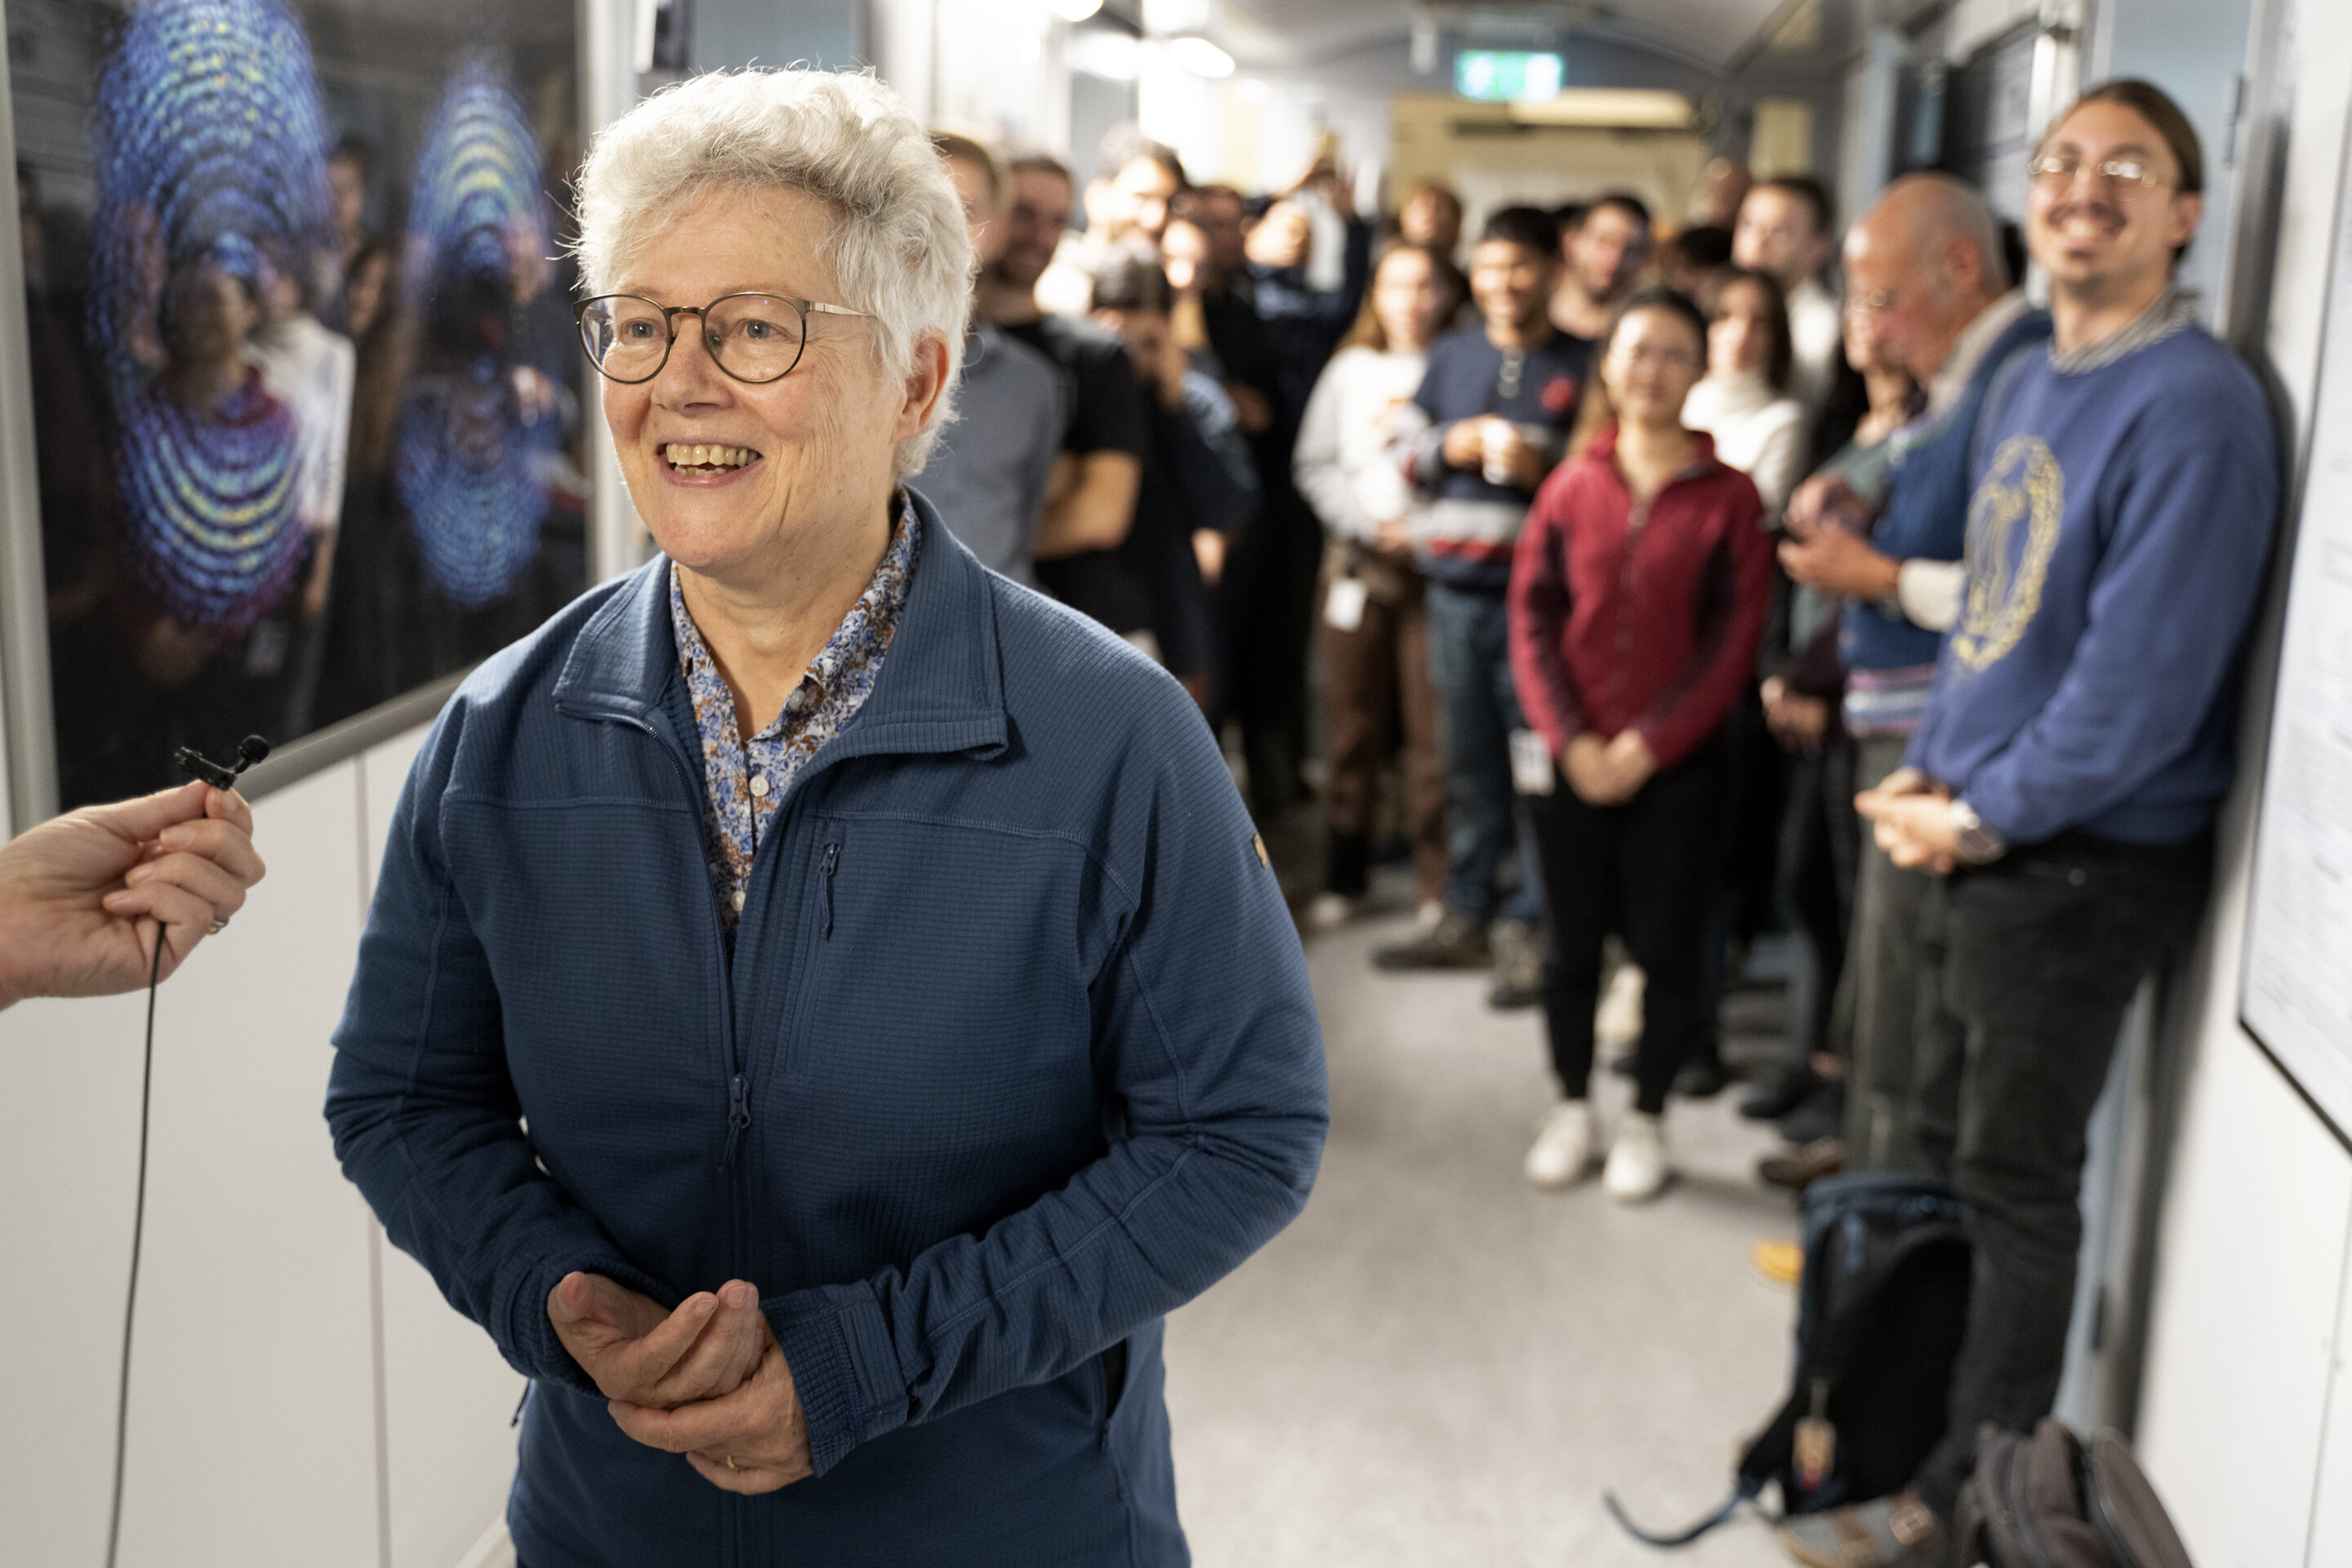
\includegraphics[width= 1\linewidth]{2}
		\caption{\small\textit{\color{timhieukhoahoc}Anne L'Huillier trả lời phỏng vấn tại Đại học Lund, Lund, Thụy Điển hôm thứ ba $3/10/2023$.}}
		\vspace*{-10pt}
	\end{figure}
%	\end{figure}
%	\begin{figure}[H]
%		\vspace*{-5pt}
%		\centering
%		\captionsetup{labelformat= empty, justification=centering}
%		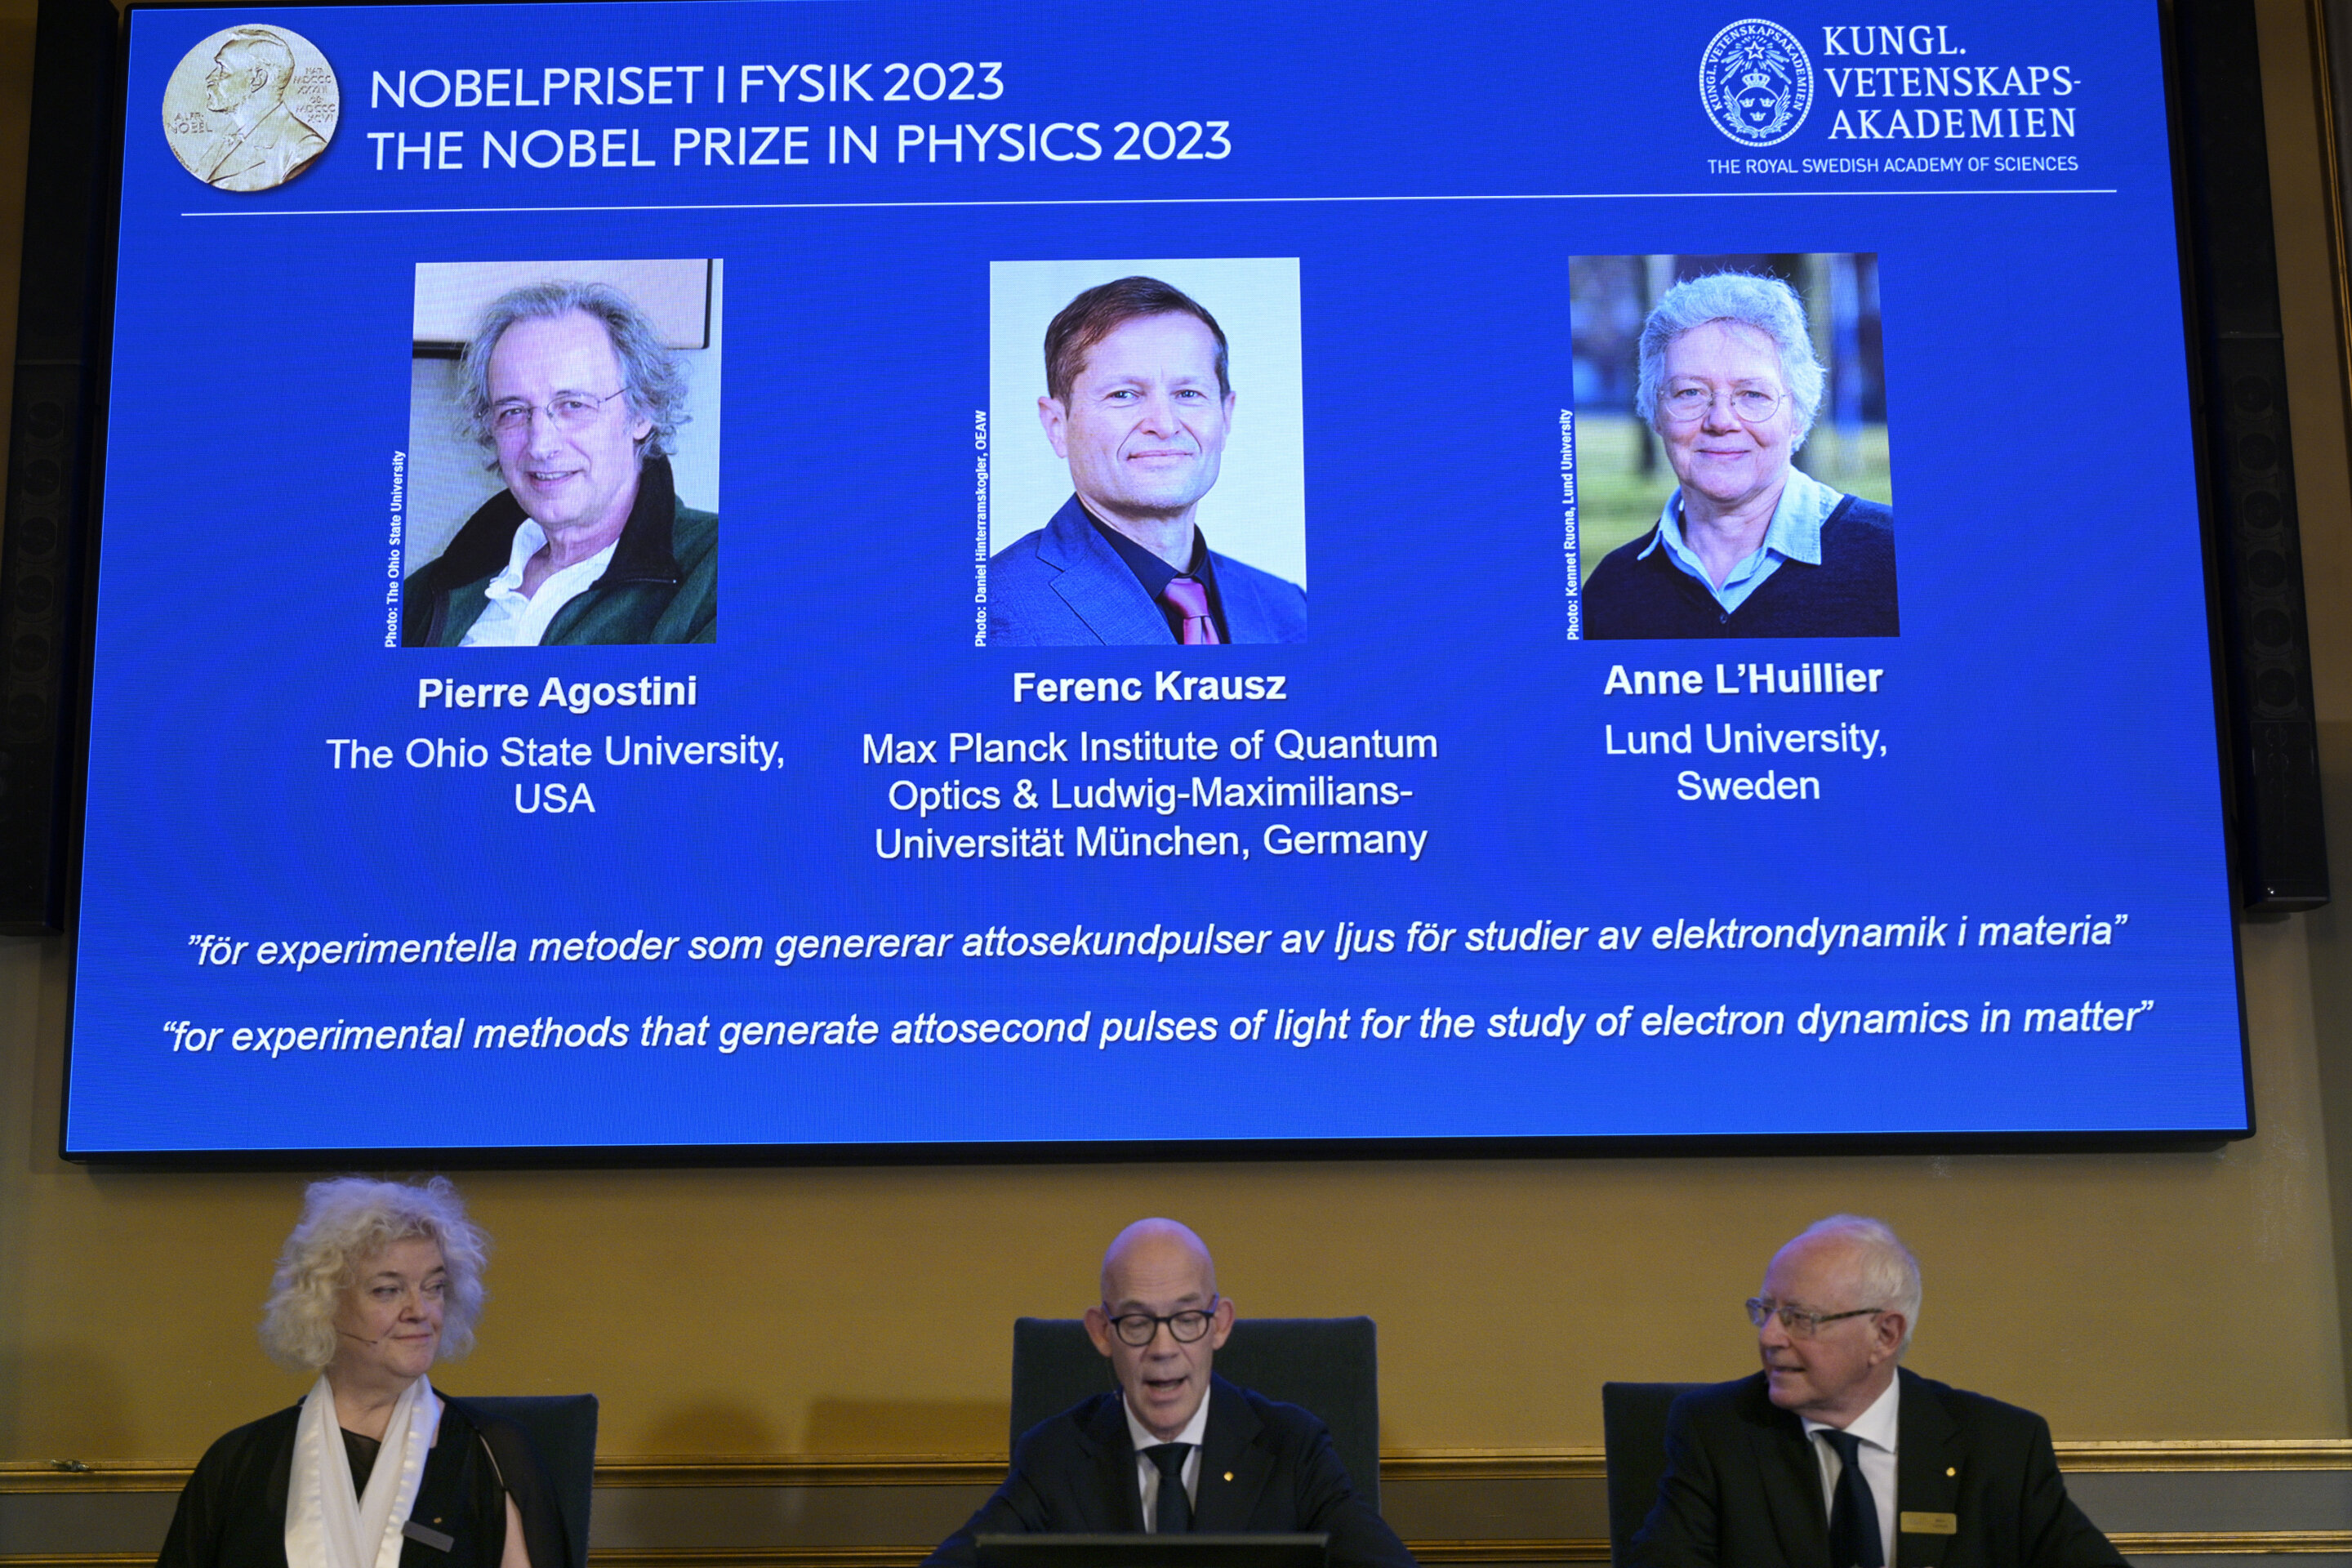
\includegraphics[width= 1\linewidth]{4}
%		%		\caption{\small\textit{\color{}}}
%		\vspace*{-15pt}
%	\end{figure}
	\textbf{\color{timhieukhoahoc}Phản ứng của ba nhà khoa học}
	\vskip 0.1cm
	Khi nhận được cuộc gọi báo tin được giải thưởng, L'Huillier đang dạy vật lý cơ bản dành cho kỹ sư cho khoảng $100$ sinh viên tại Lund; điện thoại của bà để ở chế độ im lặng và bà không nghe máy. Bà kiểm tra điện thoại trong giờ giải lao và gọi lại cho Ủy ban Giải thưởng Nobel.
	\vskip 0.1cm
	Sau đó bà quay lại dạy tiếp.
	\vskip 0.1cm
	``Lúc ấy tôi đang rất tập trung, tôi quên đi Giải Nobel và cố kết thúc bài giảng của mình," bà nói với AP. Bà kết thúc bài giảng sớm một chút để có thể trả lời họp báo công bố giải thưởng tại Viện Hàn lâm Khoa học Hoàng gia Thụy Điển ở Stockholm.
	\vskip 0.1cm
	``Đây là giải thưởng cao quý nhất và tôi thật hạnh phúc được nhận nó. Thật không thể tin được," bà nói ở buổi họp báo. ``Các bạn biết đấy, không có nhiều phụ nữ được giải này, bởi thế nó rất đặc biệt."
	\vskip 0.1cm
	Ban tổ chức giải Nobel đăng trên tài khoản mạng xã hội của mình một bức ảnh L'Huillier đang nghe điện thoại.
	\begin{figure}[H]
		\vspace*{-5pt}
		\centering
		\captionsetup{labelformat= empty, justification=centering}
		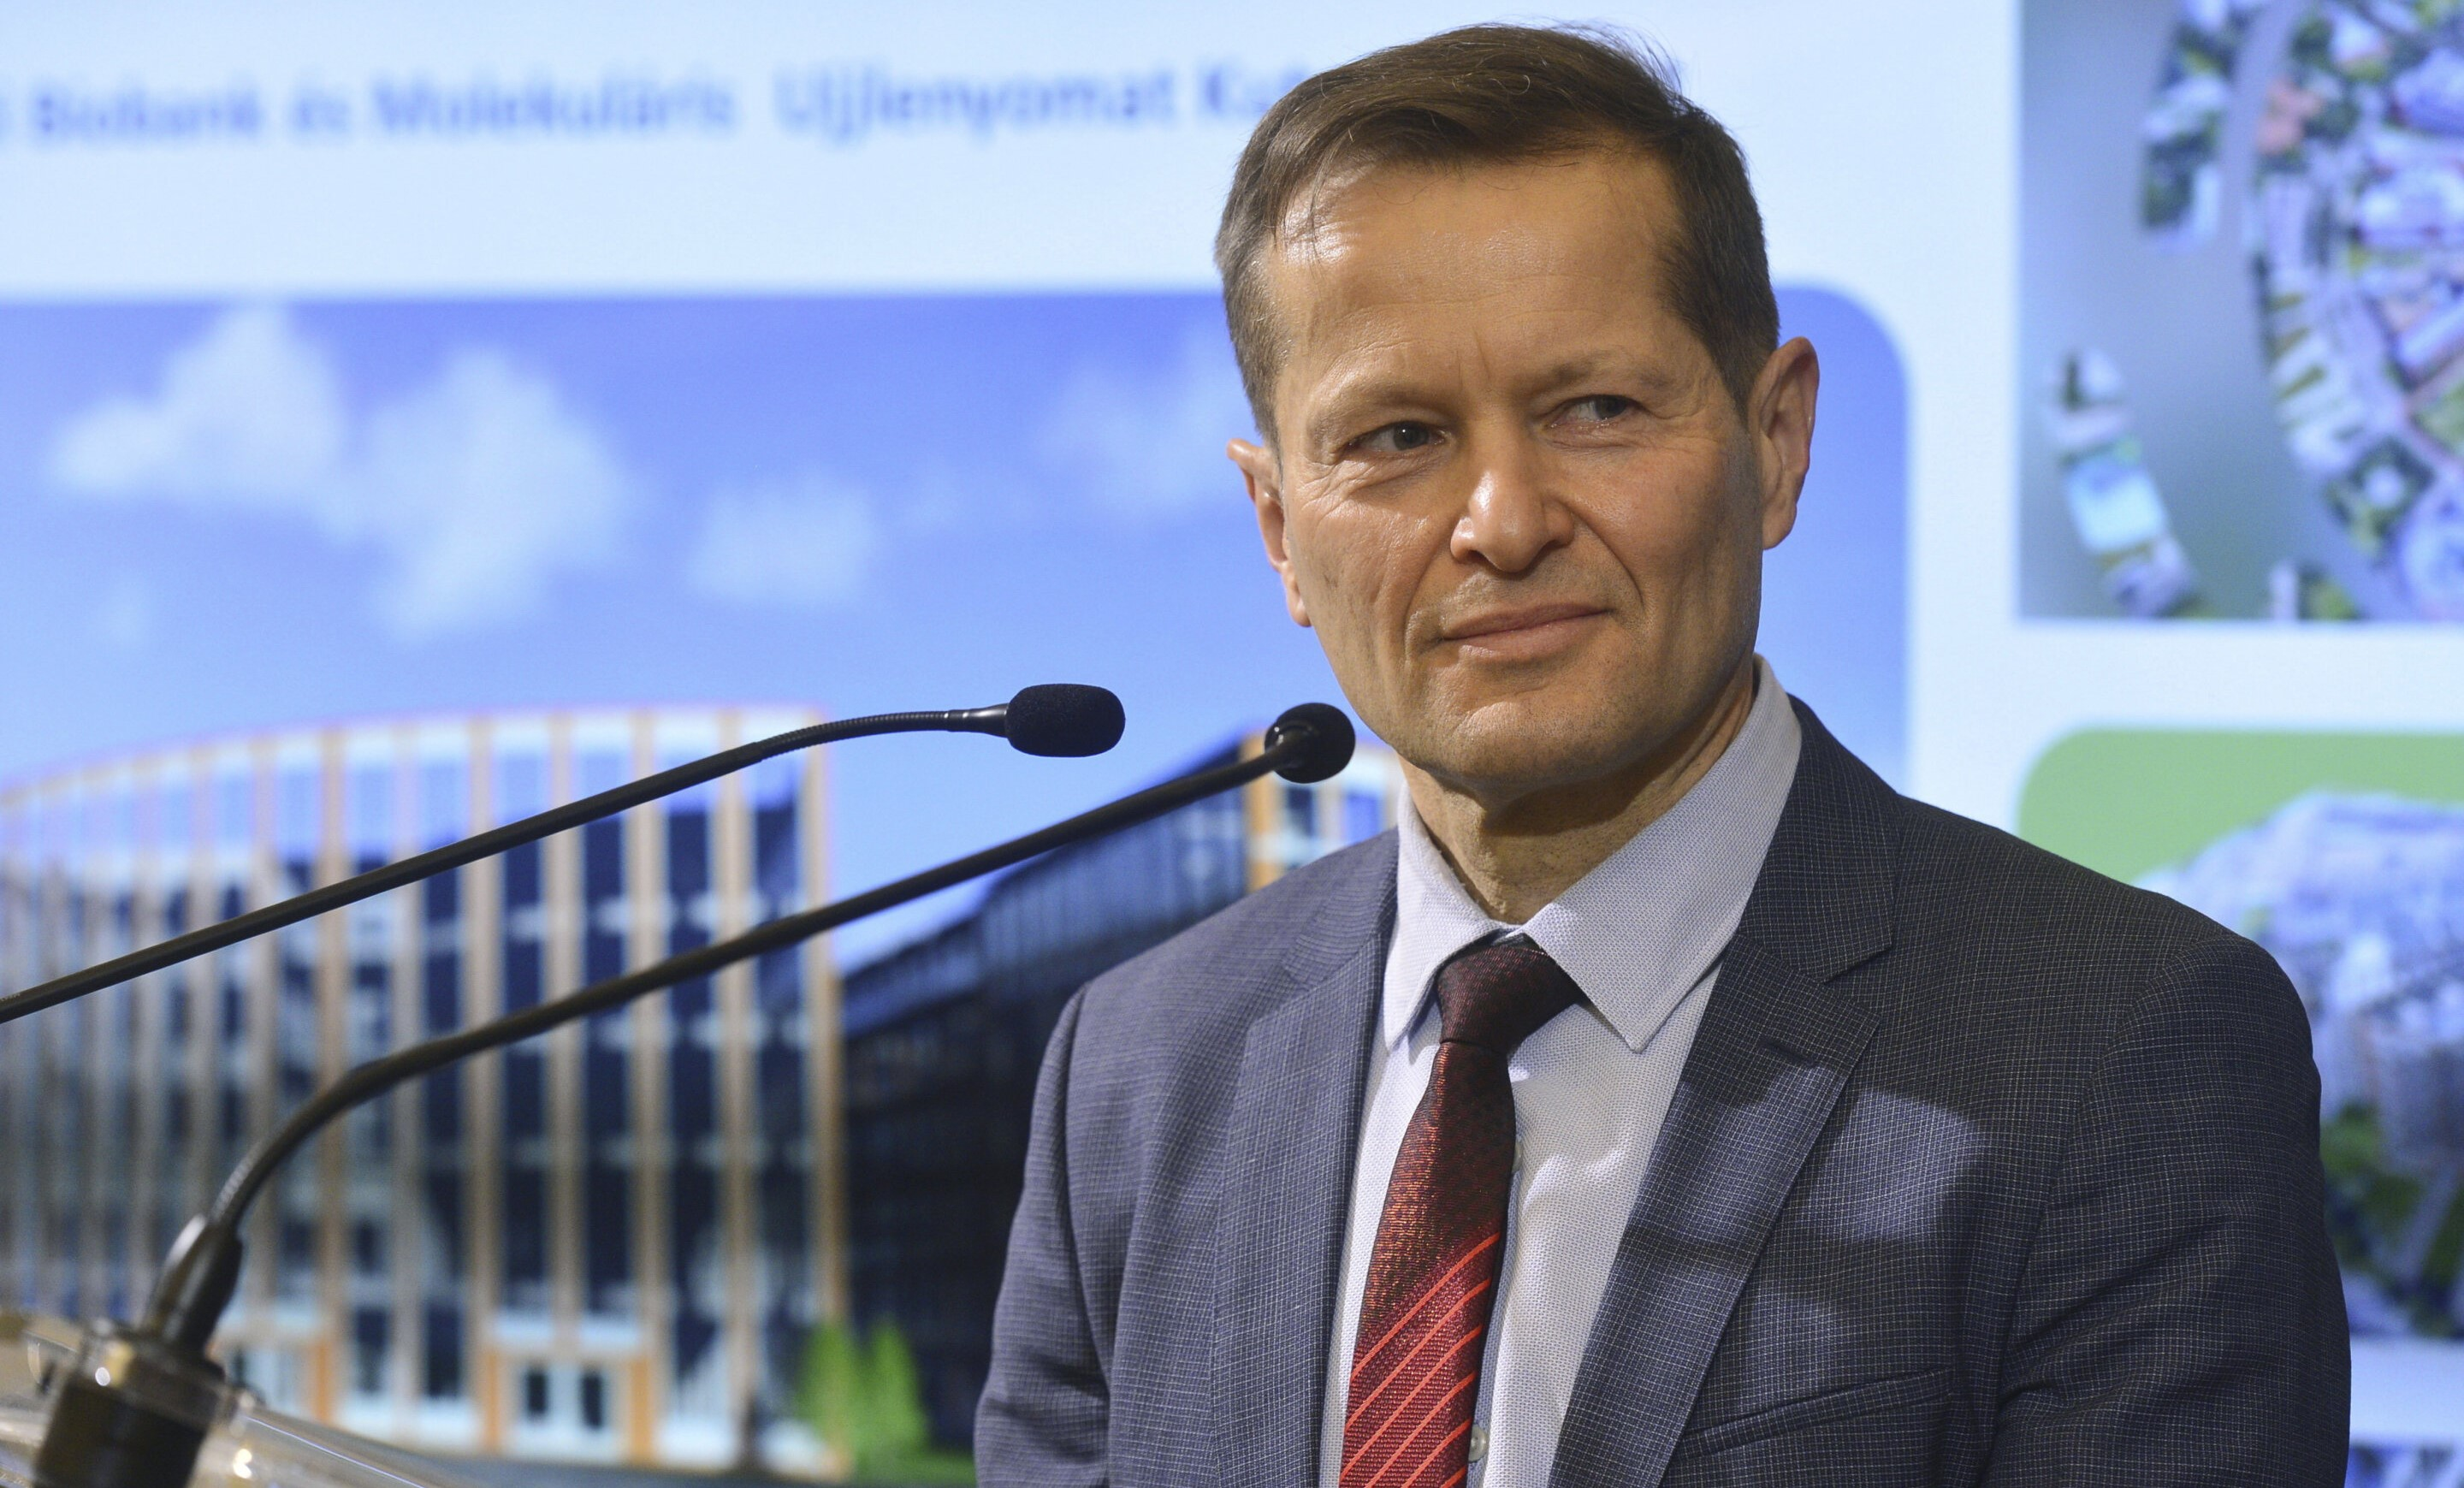
\includegraphics[width= 1\linewidth]{7}
		\caption{\small\textit{\color{timhieukhoahoc}Nhà vật lý người Hungary Ferenc Krausz.}}
		\vspace*{-10pt}
	\end{figure}
	``Cảnh báo: nhà giáo tận tâm!" bài đăng trên Twitter, nay là X, viết. ``Đến cả giải Nobel Vật lý $2023$ cũng không thể kéo Anne L'Huillier khỏi sinh viên của bà."
	\vskip 0.1cm
	Và L'Huillier cho biết khi đó vẫn phải giữ bí mật về giải thưởng nên bà không được phép giải thích với sinh viên, nhưng họ đoán được.
	\vskip 0.1cm
	Agostini, giáo sư danh dự tại Đại học Bang Ohio, khi đó đang ở Paris; Ủy ban Giải thưởng Nobel không liên lạc được với ông trước khi công bố việc ông được giải với cả thế giới.
	\vskip 0.1cm
	``Tôi không nhận được cuộc gọi nào từ ủy ban giải thưởng. Có lẽ không đúng. Tôi không biết," ông cười khi trả lời AP. ``Tôi nghĩ họ tìm tôi ở Columbus\footnote[4]{\color{timhieukhoahoc}Thủ phủ bang Ohio -- Pi.}."
	\vskip 0.1cm
	``Chắc chắn có nhiều người trẻ hơn đánh giá cao giải thưởng này hơn tôi," vị giáo sư $82$ tuổi nói đùa. ``Nó cũng tốt đấy, nhưng với tôi thì hơi muộn."
	\vskip 0.1cm
	Nhưng, ông nói thêm: ``Tôi không nghĩ mình sẽ xứng đáng nếu được trao giải sớm hơn!"
	\vskip 0.1cm
	Krausz, thuộc Viện Quang học Lượng tử Max Planck và Đại học Ludwig Maximilian tại Munich, nói với các phóng viên rằng ông bị choáng ngợp.
	\vskip 0.1cm
	``Từ $11$ giờ sáng đến giờ tôi vẫn đang nghĩ xem mình đang ở trong hiện thực hay trong một giấc mơ dài," nhà vật lý $61$ tuổi nói.
	\vskip 0.1cm
	Cuộc gọi từ ủy ban giải thưởng được hiển thị ``không có ID người gọi" và thường thì Krausz không nghe những cuộc gọi như vậy, nhưng lần này, ông ``nghĩ rằng mình sẽ thử nghe, và rõ ràng không thể dập máy ngay."
	\vskip 0.1cm
	Năm ngoái, cùng với nhà khoa học Paul Corkum của Đại học Ottawa, Krausz và L'Huillier được trao giải thưởng vật lý cao quý Wolf vì những công trình của họ. Giải Nobel chỉ được trao cho không quá ba người, và Krausz nói rằng thật đáng tiếc khi nó không thể được trao cho Corkum.
	\vskip 0.1cm
	Corkum là chìa khóa đối với cách đo các xung laser xảy ra trong tích tắc, và điều này mang tính cốt yếu, Krausz nói.
	\begin{figure}[H]
		\vspace*{-5pt}
		\centering
		\captionsetup{labelformat= empty, justification=centering}
		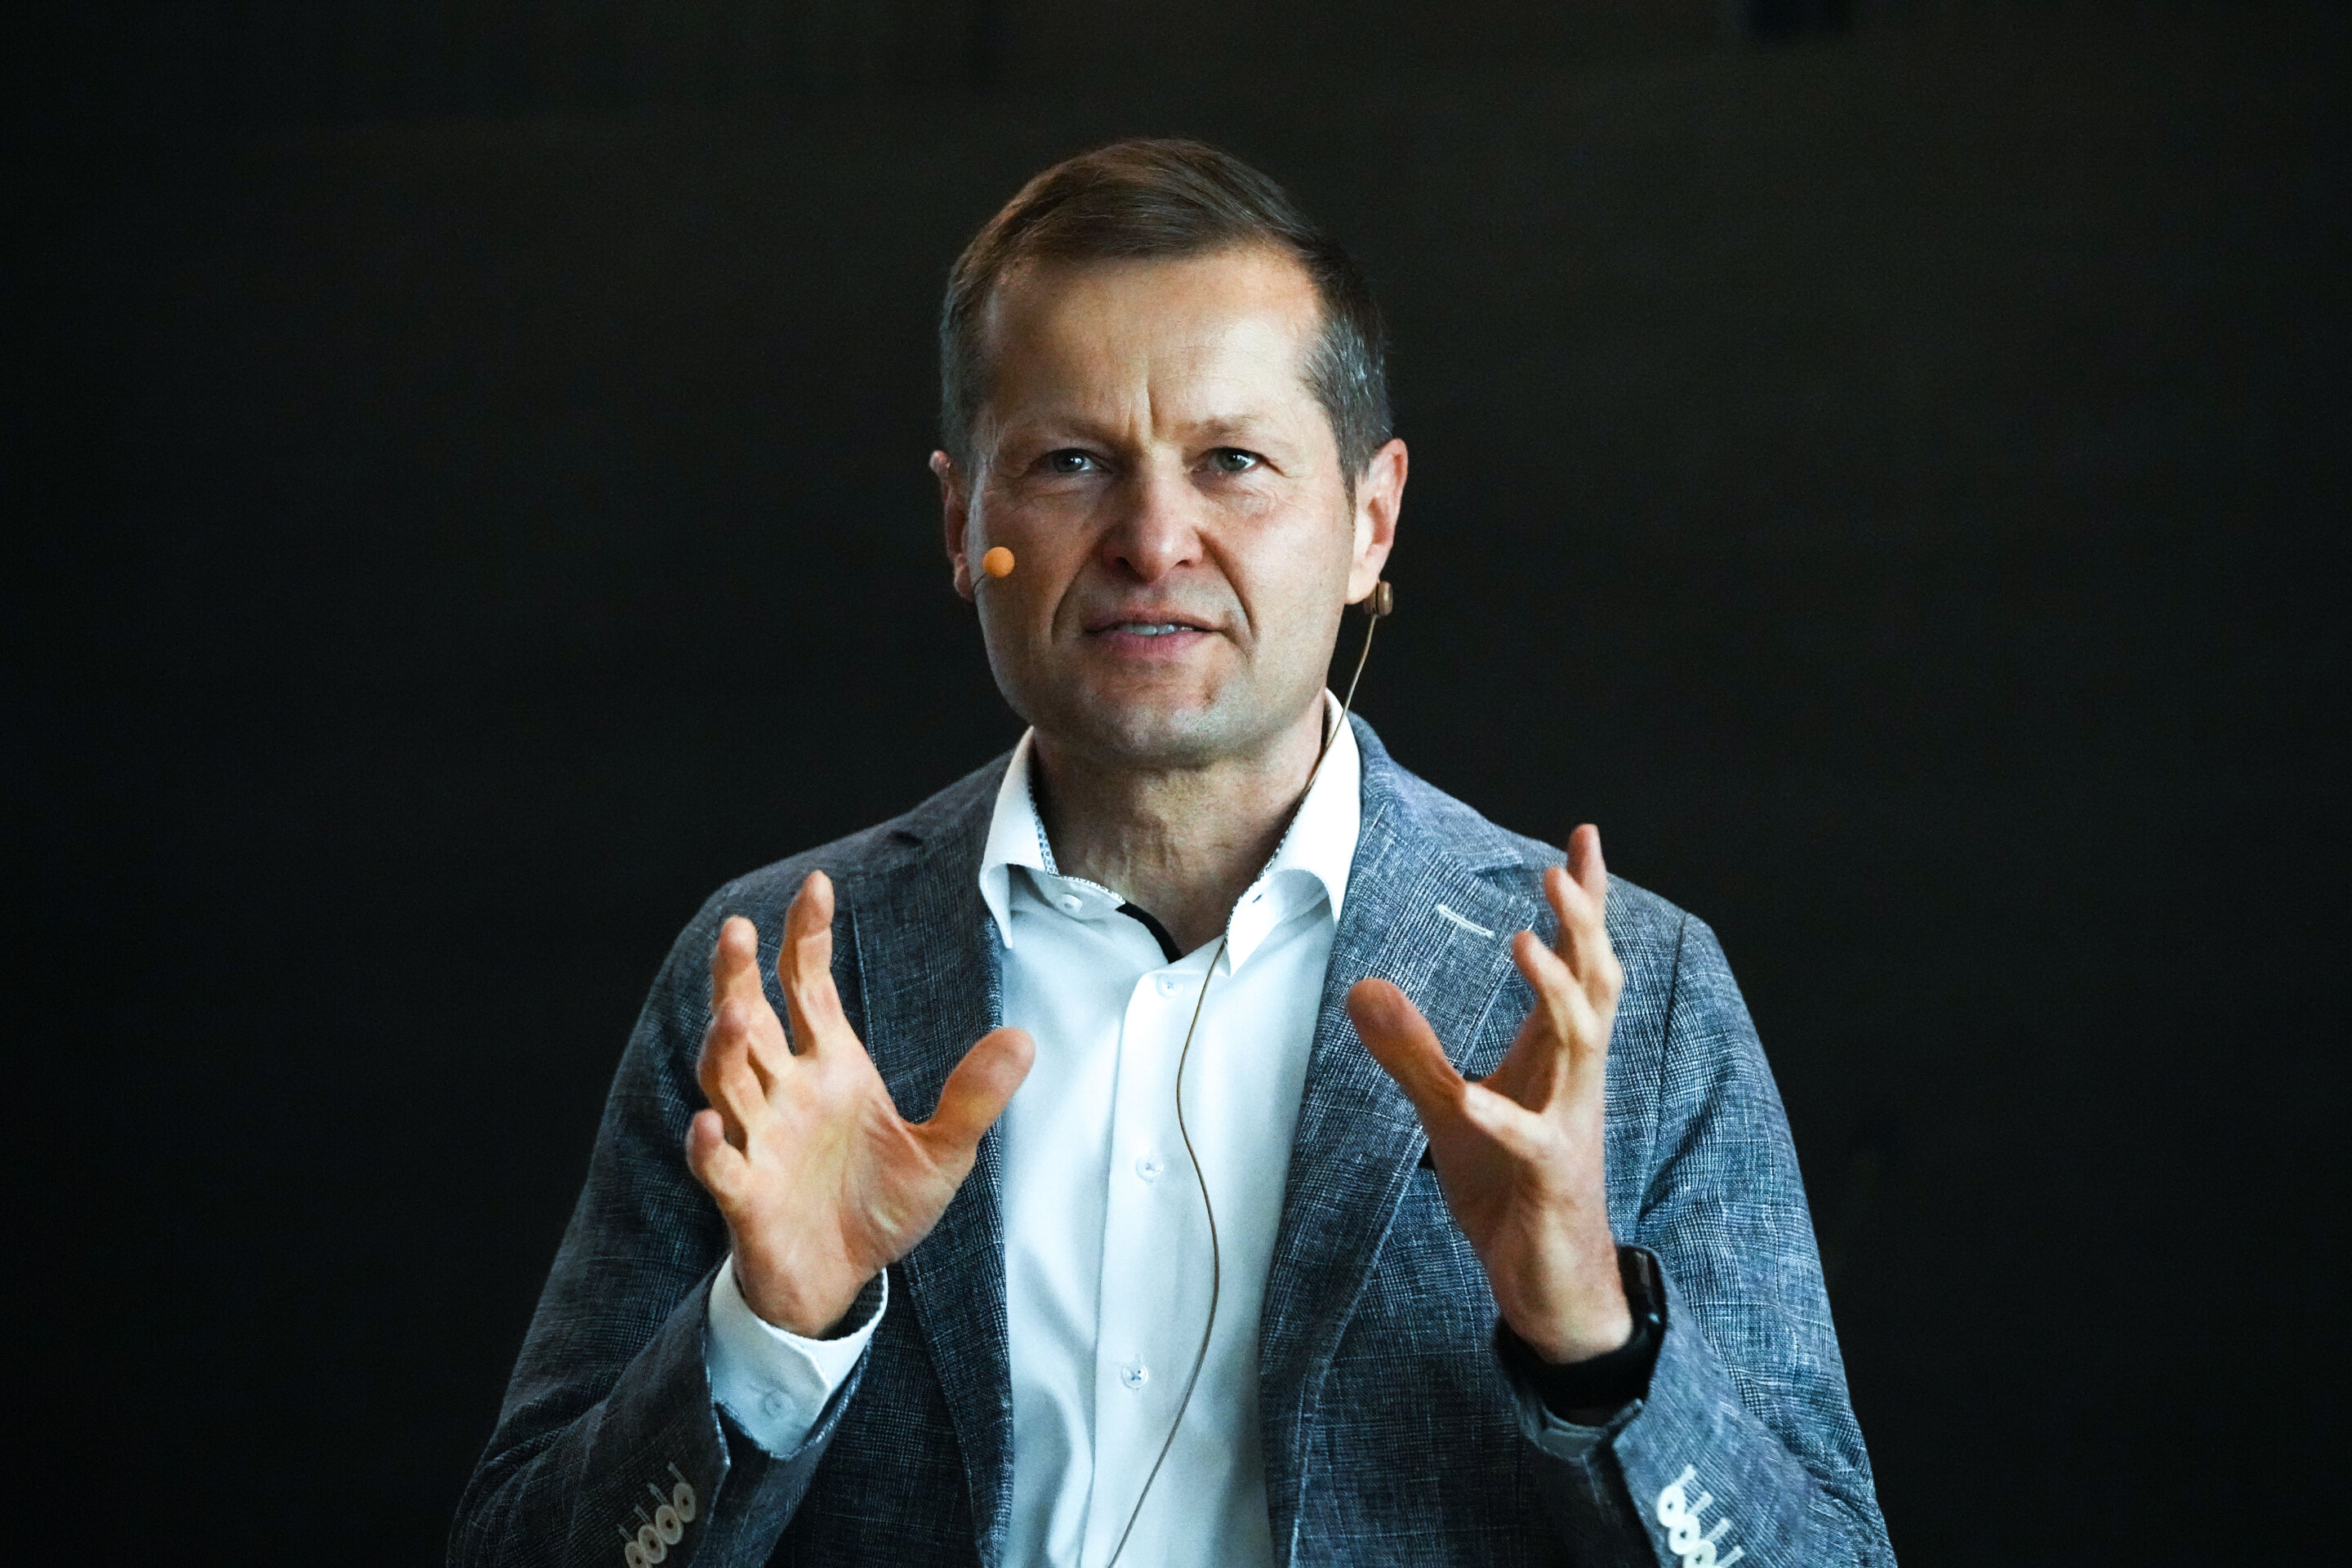
\includegraphics[width= 1\linewidth]{5}
		\caption{\small\textit{\color{timhieukhoahoc}Ferenc Krausz trong một buổi thuyết trình tại Viện Quang học Lượng tử Max Planck, Munich, Đức hôm thứ ba $3/10/2023$.}}
		\vspace*{-15pt}
	\end{figure}
	Giải Nobel có giá trị tiền thưởng khoảng $1$ triệu đô--la Mỹ, được trao theo di chúc của người sáng lập ra nó, nhà phát minh người Thụy Điển Alfred Nobel.
	\vskip 0.1cm
	Giải Nobel Vật lý được công bố một ngày sau khi hai nhà khoa học được giải Nobel Y học -- Sinh lý học vì những khám phá giúp tạo ra vaccine mRNA cho COVID--$19$.
	\vskip 0.1cm
	\textbf{\color{timhieukhoahoc}Thông báo của Ủy ban Giải thưởng Nobel:}
	\vskip 0.1cm
	Viện Hàn lâm Khoa học Hoàng gia Thụy Điển quyết định trao giải Nobel Vật lý $2023$ cho
	\vskip 0.1cm
	\textbf{\color{timhieukhoahoc}Pierre Agostini}, Đại học Bang Ohio, Columbus, Mỹ
	\vskip 0.1cm
	\textbf{\color{timhieukhoahoc}Ferenc Krausz},  Viện Quang học Lượng tử Max Planck, Garching và Đại học Ludwig Maximilian tại Munich, Đức
	\vskip 0.1cm
	\textbf{\color{timhieukhoahoc}Anne L'Huillier}, Đại học Lund, Thụy Điển
	\vskip 0.1cm
	``vì các phương pháp thực nghiệm tạo ra các xung ánh sáng atto giây nhằm nghiên cứu động lực học của electron trong vật chất".
	\begin{figure}[H]
		\vspace*{-5pt}
		\centering
		\captionsetup{labelformat= empty, justification=centering}
		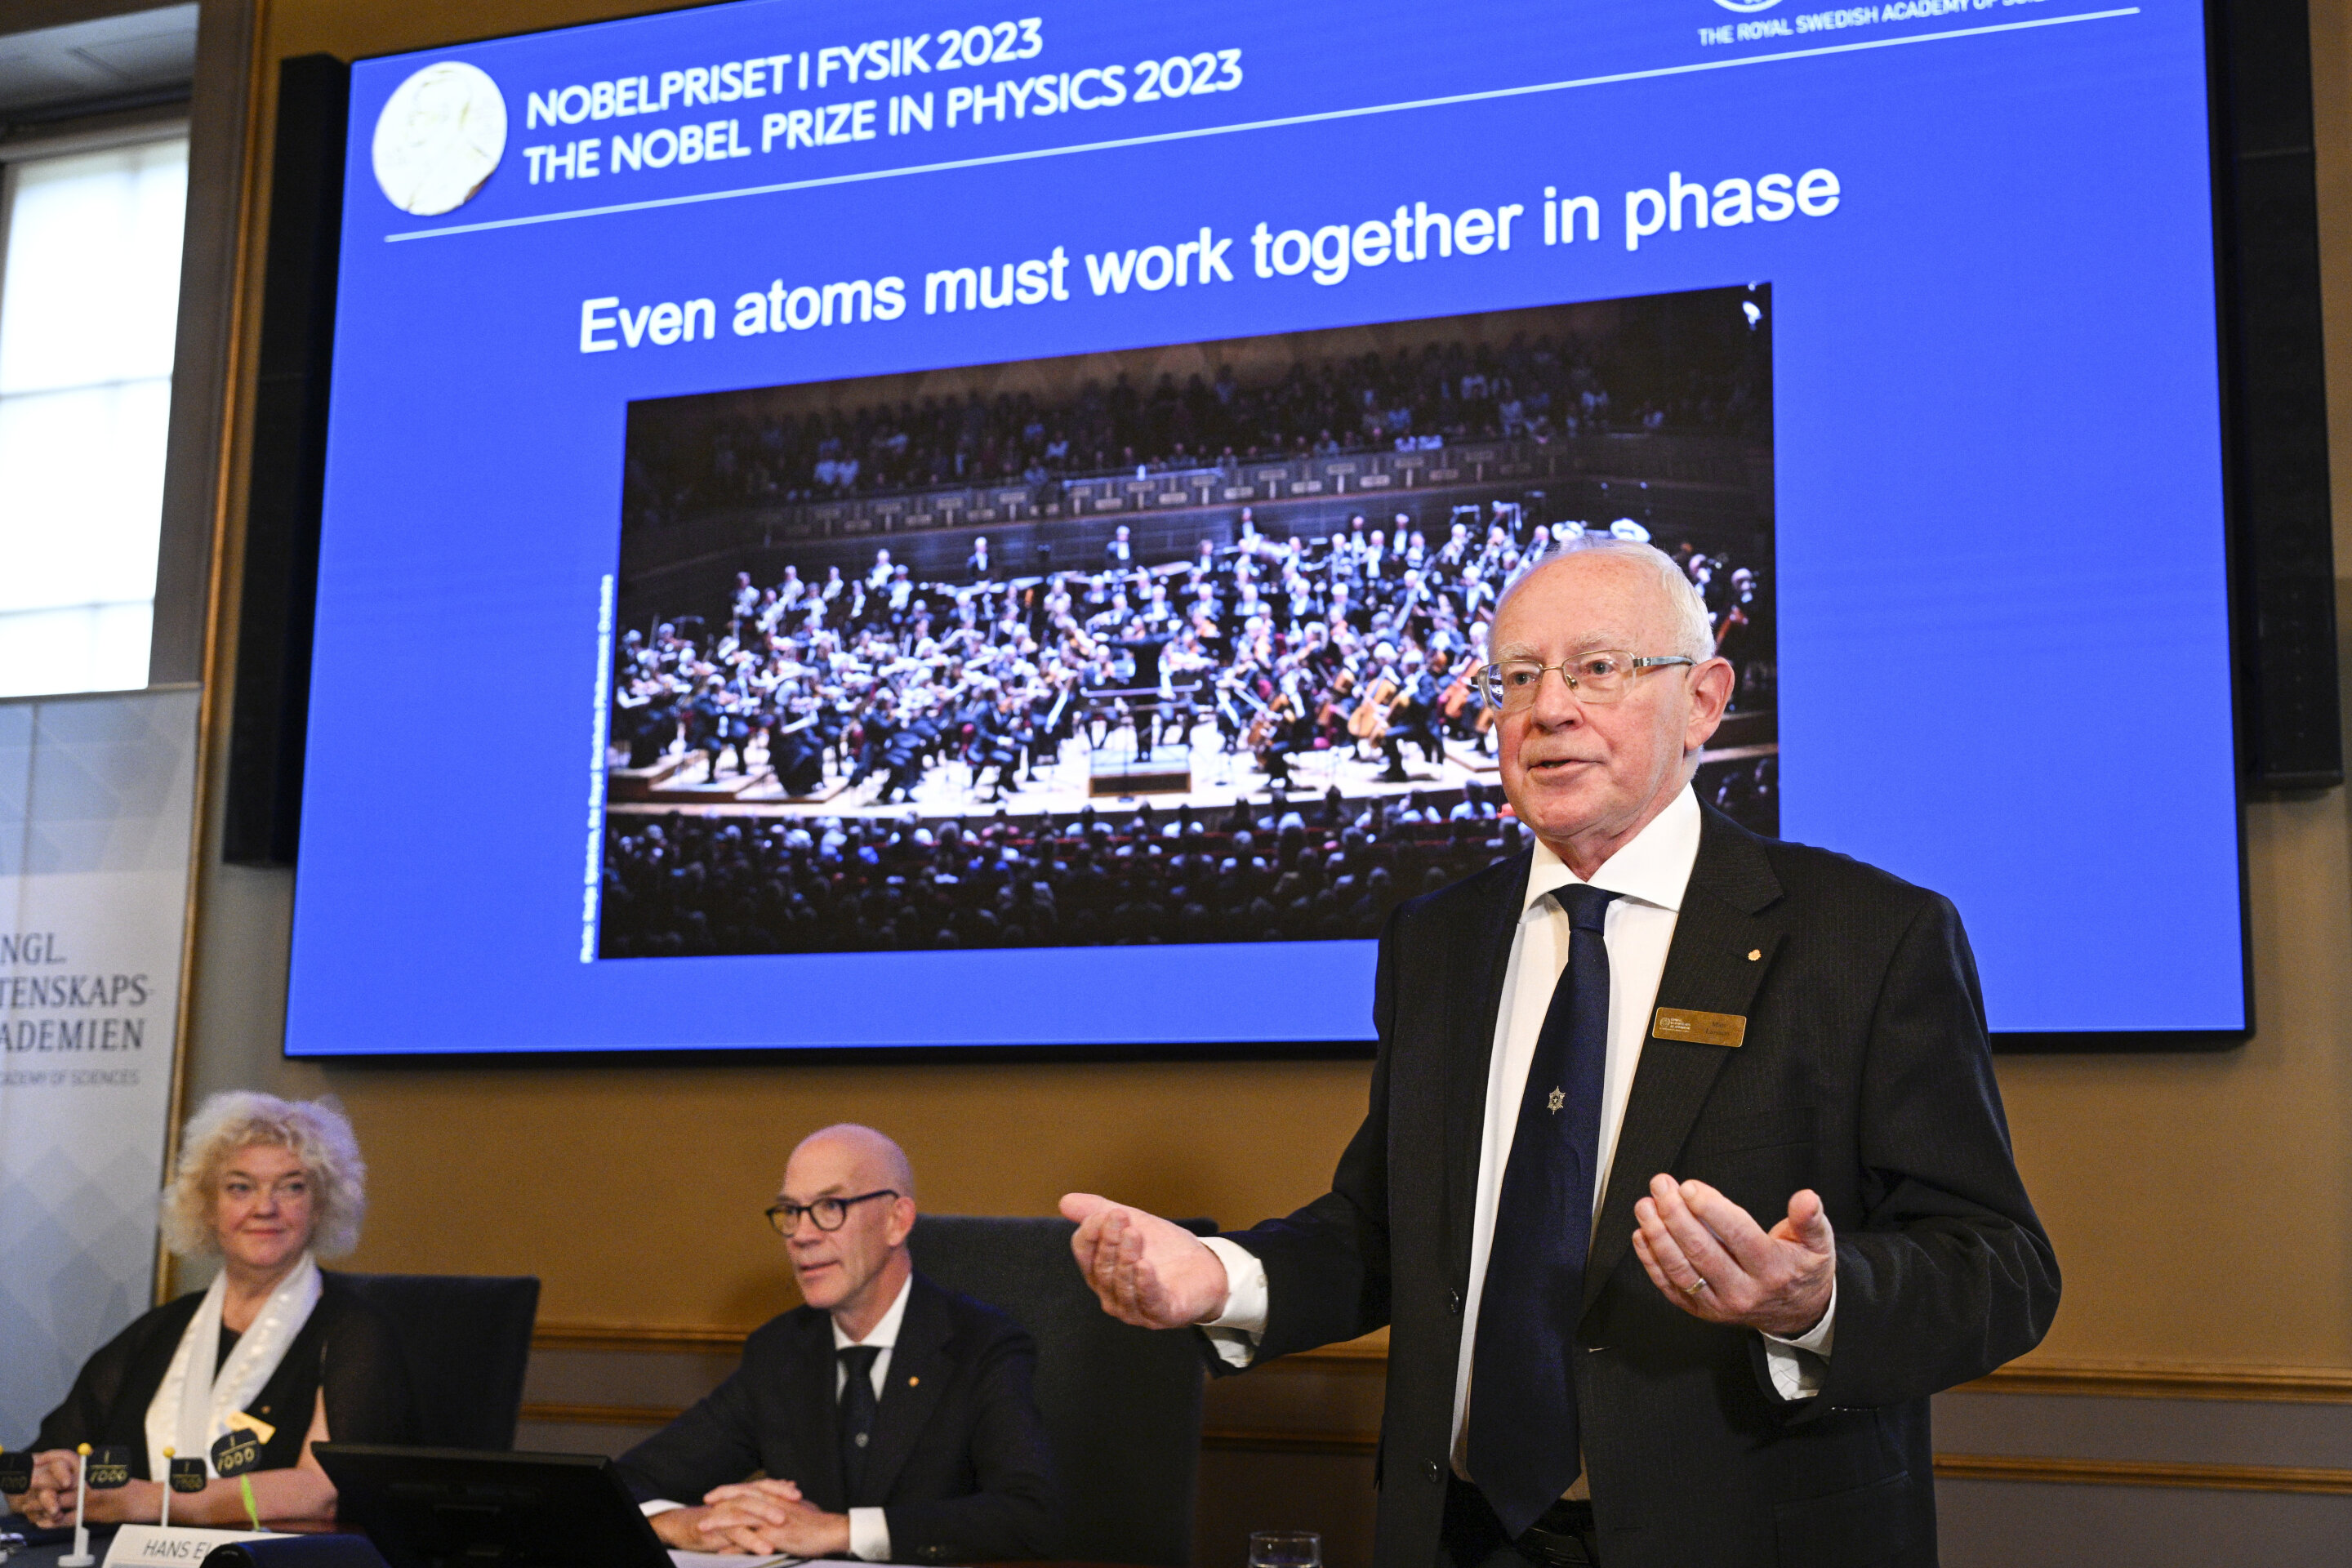
\includegraphics[width= 1\linewidth]{9}
%		\caption{\small\textit{\color{}}}
		\vspace*{-15pt}
	\end{figure}
	\textbf{\color{timhieukhoahoc}Thí nghiệm với ánh sáng bắt được những khoảnh khắc ngắn nhất}
	\vskip 0.1cm
	Ba nhà khoa học được giải Nobel Vật lý $2023$ được vinh danh vì những thí nghiệm cung cấp cho nhân loại những công cụ mới để khám phá thế giới của electron bên trong nguyên tử và phân tử. Pierre Agostini, Ferenc Krausz và Anne L'Huillier đã trình bày một cách tạo ra những xung ánh sáng cực ngắn có thể được dùng để đo các quá trình rất nhanh, trong đó electron di chuyển hoặc thay đổi năng lượng.
	\vskip 0.1cm
	Các sự kiện tốc độ cao chảy vào với nhau khi được quan sát bởi con người, giống như một đoạn phim gồm những hình ảnh tĩnh được nhìn thấy như chuyển động liên tục. Nếu muốn tìm hiểu về những sự kiện thực sự ngắn ngủi, chúng ta cần những công nghệ đặc biệt. Trong thế giới của electron, những thay đổi xảy ra chỉ trong vài chục atto giây -- một atto giây là một khoảng thời gian rất ngắn, ngắn đến nỗi số atto giây trong một giây bằng số giây tính từ khi vũ trụ ra đời.
	\vskip 0.1cm
	Những thí nghiệm của các nhà khoa học được giải đã tạo ra các xung ánh sáng ngắn đến cỡ atto giây, từ đó cho thấy các xung này có thể được sử dụng để cung cấp những hình ảnh về các quá trình bên trong nguyên tử và phân tử.
	\vskip 0.1cm
	Năm $1987$, Anne L'Huillier phát hiện thấy nhiều sóng hài bậc cao khác nhau xuất hiện khi bà truyền laser hồng ngoại qua một khí hiếm. Mỗi sóng hài bậc cao là một sóng ánh sáng mà mỗi chu kỳ của ánh sáng laser bằng một bội của chu kỳ của sóng hài. Chúng được sinh ra do laser tương tác với các phân tử khí; nó cung cấp năng lượng cho một số electron, và năng lượng dư thừa này được phát lại dưới dạng ánh sáng. Anne L'Huillier tiếp tục tìm hiểu hiện tượng này, đặt nền móng cho những đột phá tiếp theo.
	\vskip 0.1cm
	Năm $2001$, Pierre Agostini thành công trong việc tạo ra và nghiên cứu một chuỗi các xung ánh sáng liên tiếp, trong đó mỗi xung chỉ dài $250$ atto giây. Cùng lúc đó, Ferenc Krausz đang tiến hành một loại thí nghiệm khác, cho phép tách riêng một xung ánh sáng dài $650$ atto giây.
	\vskip 0.1cm
	Đóng góp của các nhà khoa học được giải cho phép nghiên cứu các quá trình diễn ra rất nhanh, mà trước đó không thể theo kịp.
	\vskip 0.1cm
	``Giờ chúng ta có thể mở cánh cửa vào thế giới của electron. Vật lý atto giây cho chúng ta cơ hội hiểu được các cơ chế do electron chi phối. Bước tiếp theo sẽ là sử dụng chúng," Eva Olsson, chủ tịch Ủy ban Giải thưởng Nobel về Vật lý, nói.
	\vskip 0.1cm
	Có nhiều ứng dụng tiềm năng trong những lĩnh vực khác nhau. Chẳng hạn, trong điện tử, việc hiểu và điều khiển được hành vi của electron trong vật liệu là rất quan trọng. Các xung atto giây cũng có thể được dùng để nhận dạng các phân tử khác nhau, thí dụ trong chẩn đoán y tế.
	\begin{figure}[H]
		\vspace*{-5pt}
		\centering
		\captionsetup{labelformat= empty, justification=centering}
		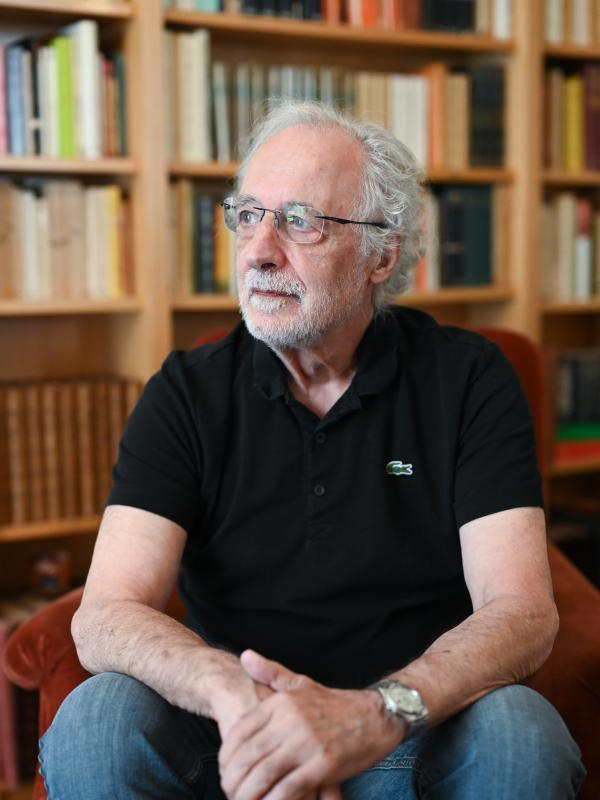
\includegraphics[width= 1\linewidth]{8}
		\caption{\small\textit{\color{timhieukhoahoc}Pierre Agostini, ảnh tại trang web khoa Vật lý, Đại học Bang Ohio.}}
		\vspace*{-10pt}
	\end{figure}
	\textbf{\color{timhieukhoahoc}Electron trong xung ánh sáng}
	\vskip 0.1cm
	Qua các thí nghiệm của mình, ba nhà khoa học được giải năm nay đã tạo được những chớp sáng đủ ngắn để chụp được chuyển động vô cùng nhanh của electron. Anne L'Huillier phát hiện ra một hiệu ứng mới từ tương tác của ánh sáng laser với các nguyên tử khí. Pierre Agostini và Ferenc Krausz cho thấy hiệu ứng này có thể được dùng để tạo ra những xung ánh sáng ngắn hơn những cái có thể được tạo ra trước đó.
	\vskip 0.1cm
	Một con chim ruồi có thể đập cánh $80$ lần mỗi giây. Chúng ta chỉ có thể nhận thấy tiếng vù vù và chuyển động mờ mờ. Với giác quan của con người, chuyển động nhanh bị mờ vào với nhau, và những sự kiện cực ngắn là không thể quan sát. Chúng ta cần đến những biện pháp công nghệ để chụp hoặc mô tả được những khoảnh khắc rất ngắn đó.
	\vskip 0.1cm
	Kỹ thuật chụp ảnh tốc độ cao và ánh sáng nhấp nháy cho phép chụp được hình ảnh chi tiết của những hiện tượng thoáng qua. Một bức ảnh rõ nét chụp một con chim ruồi đang bay đòi hỏi thời gian phơi sáng ngắn hơn nhiều so với một nhịp đập cánh của nó.
	\vskip 0.1cm
	Sự kiện càng nhanh, thời gian chụp ảnh phải càng ngắn để chụp được đúng khoảnh khắc.
	\vskip 0.1cm
	Nguyên lý tương tự được áp dụng cho tất cả các phương pháp để đo hoặc mô tả các quá trình nhanh; mọi phép đo phải được thực hiện nhanh hơn khoảng thời gian để hệ thống được quan sát trải qua một thay đổi nhận biết được, bằng không kết quả sẽ không rõ. Các nhà khoa học được giải năm nay đã tiến hành các thí nghiệm chỉ ra một phương pháp tạo ra các xung ánh sáng đủ ngắn để chụp được hình ảnh về các quá trình bên trong nguyên tử và phân tử.
	\vskip 0.1cm
	Thang thời gian tự nhiên của nguyên tử là cực kỳ nhỏ. Trong một phân tử, các nguyên tử có thể di chuyển và quay trong một phần triệu tỷ giây, hay femto giây\footnote[5]{\color{timhieukhoahoc}$1$ femto giây $= 10^{-15}$ giây -- Pi.} . Những chuyển động này có thể được nghiên cứu với những xung ngắn nhất mà một tia laser có thể tạo ra -- tuy nhiên, khi cả nguyên tử di chuyển, thang thời gian được xác định bởi hạt nhân to và nặng, vốn cực kỳ chậm so với ánh sáng và các electron nhanh nhẹn.
	\vskip 0.1cm
	Khi electron di chuyển trong nguyên tử và phân tử, chúng nhanh đến nỗi các thay đổi bị mờ sau chỉ một femto giây. Trong thế giới của electron, vị trí và năng lượng thay đổi với tốc độ từ khoảng một đến một vài trăm atto giây, tức một phần tỷ tỷ giây.
	\vskip 0.1cm
	Một atto giây ngắn đến nỗi số atto giây trong một giây bằng số giây từ khi vũ trụ sinh ra, $13{,}8$ tỷ năm trước, đến hiện tại. Để dễ hình dung, ta có thể tưởng tượng một chớp sáng đi từ một đầu căn phòng đến bức tường đối diện: nó mất mười tỷ atto giây.
	\vskip 0.1cm
	Trong một thời gian dài, một femto giây được coi là giới hạn của những chớp sáng tạo ra được.
	\vskip 0.1cm
	Việc cải tiến công nghệ sẵn có không đủ để thấy được các quá trình diễn ra trong thang thời gian ngắn đến kinh ngạc của electron; cần có một cái gì đó hoàn toàn mới. Các nhà khoa học được giải năm nay đã thực hiện những thí nghiệm mở ra lĩnh vực vật lý atto giây mới mẻ.
	\vskip 0.1cm
	\textbf{\color{timhieukhoahoc}Xung ngắn hơn nhờ các sóng hài bậc cao}
	\vskip 0.1cm
	Ánh sáng gồm những sóng -- dao động trong trường điện từ -- di chuyển trong chân không nhanh hơn mọi thứ. Sóng ánh sáng có các bước sóng khác nhau, tương đương với màu sắc khác nhau. Thí dụ, bước sóng của ánh sáng đỏ dài khoảng $700$ nm, tức khoảng một phần trăm bề rộng của một sợi tóc, và nó lặp đi lặp lại khoảng bốn trăm ba mươi nghìn tỷ lần mỗi giây. Chúng ta có thể nghĩ về xung ánh sáng ngắn nhất có thể như độ dài một chu kỳ của sóng ánh sáng, tính từ khi nó ở trên đỉnh, đi xuống đáy, rồi quay lại điểm bắt đầu. Trong trường hợp này, bước sóng dùng trong một hệ laser thông thường không thể nào đạt dưới femto giây, vì vậy trong những năm $1980$, đây được xem là một giới hạn cứng cho độ ngắn của một xung ánh sáng.
	\vskip 0.1cm
	Về mặt toán học, có thể chứng minh được rằng có thể tạo được mọi dạng sóng nếu có đủ những sóng có bước sóng và biên độ thích hợp. Bí quyết tạo ra xung atto giây là có thể tạo ra những xung ngày càng ngắn bằng cách kết hợp các bước sóng ngày càng ngắn.
	\vskip 0.1cm
	Để quan sát chuyển động của electron ở thang nguyên tử, cần các xung ánh sáng đủ ngắn, nghĩa là cần kết hợp nhiều sóng ngắn với bước sóng khác nhau.
	\vskip 0.1cm
	Để thêm bước sóng mới cho ánh sáng, cần nhiều hơn là một laser; chìa khóa dẫn đến khoảnh khắc ngắn nhất quan sát được từ trước đến nay là một hiện tượng xảy ra khi laser đi qua một chất khí. Ánh sáng tương tác với các nguyên tử khí và gây ra sóng hài bậc cao -- những sóng hoàn thành nhiều chu kỳ tương ứng với mỗi chu kỳ của sóng ban đầu. Chúng ta có thể so sánh hiện tượng này với âm bội tạo ra đặc tính của một âm thanh, giúp ta nghe được sự khác biệt của cùng một nốt khi được chơi trên ghi--ta và khi được chơi trên pi--a--nô.
	\vskip 0.1cm
	Năm $1987$, Anne L'Huillier và các đồng nghiệp tại một phòng thí nghiệm ở Pháp đã tạo được sóng hài bậc cao bằng cách sử dụng một laser hồng ngoại chiếu qua một khí hiếm. Laser hồng ngoại này tạo ra các sóng hài bậc cao ngày càng mạnh hơn so với những laser bước sóng ngắn được dùng trong các thí nghiệm trước đó. Trong thí nghiệm này, họ đã quan sát được nhiều sóng hài bậc cao với cường độ tương tự nhau.
	\vskip 0.1cm
	Trong một loạt các bài báo trong những năm $1990$, L'Huillier tiếp tục tìm hiểu hiệu ứng này, cả khi bà đã chuyển đến Đại học Lund. Những kết quả của bà đóng góp cho hiểu biết lý thuyết về hiện tượng này, đặt nền móng cho thí nghiệm đột phá tiếp theo.
	\vskip 0.1cm
	\textbf{\color{timhieukhoahoc}Electron thoát ly tạo sóng hài bậc cao}
	\vskip 0.1cm
	Khi ánh sáng laser đi qua chất khí và tác động lên các nguyên tử khí, nó tạo ra những dao động điện từ làm biến dạng điện trường giữ các electron quanh hạt nhân nguyên tử. Do đó, electron có thể thoát khỏi nguyên tử. Tuy nhiên, điện trường của ánh sáng dao động liên tục và khi nó đổi hướng, một electron đã thoát ra có thể chạy ngược về hạt nhân nguyên tử của nó. Trong chuyến du hành của mình, electron nhận thêm nhiều năng lượng từ điện trường của ánh sáng laser, và để liên kết lại với hạt nhân, nó cần giải phóng năng lượng dư thừa dưới dạng xung ánh sáng. Những xung phát ra từ electron này chính là thứ tạo ra sóng hài bậc cao được quan sát trong thí nghiệm.
	\vskip 0.1cm
	Năng lượng của ánh sáng gắn liền với bước sóng của nó. Năng lượng trong sóng hài bậc cao được phát ra tương đương với ánh sáng cực tím, vốn có bước sóng ngắn hơn ánh sáng nhìn thấy bằng mắt thường. Vì năng lượng đến từ dao động của laser, dao động của sóng hài bậc cao tỷ lệ một cách đẹp đẽ với bước sóng của xung laser ban đầu. Tương tác của ánh sáng với nhiều nguyên tử khác nhau cho kết quả là nhiều sóng ánh sáng khác nhau với những bộ bước sóng riêng.
	\vskip 0.1cm
	Khi đã được tạo ra, những sóng hài bậc cao này tương tác với nhau. Ánh sáng mạnh hơn khi các đỉnh sóng trùng nhau, và yếu hơn khi đỉnh của sóng này trùng với đáy của sóng khác. Trong những điều kiện thích hợp, các sóng hài bậc cao trùng khít với nhau, tạo ra một chuỗi các xung cực tím, mỗi xung dài vài trăm atto giây. Các nhà vật lý hiểu được lý thuyết đằng sau hiện tượng này từ những năm $1990$, nhưng đột phá trong việc xác định và kiểm nghiệm các xung này đến vào năm $2001$.
	\begin{figure}[H]
		\vspace*{-5pt}
		\centering
		\captionsetup{labelformat= empty, justification=centering}
		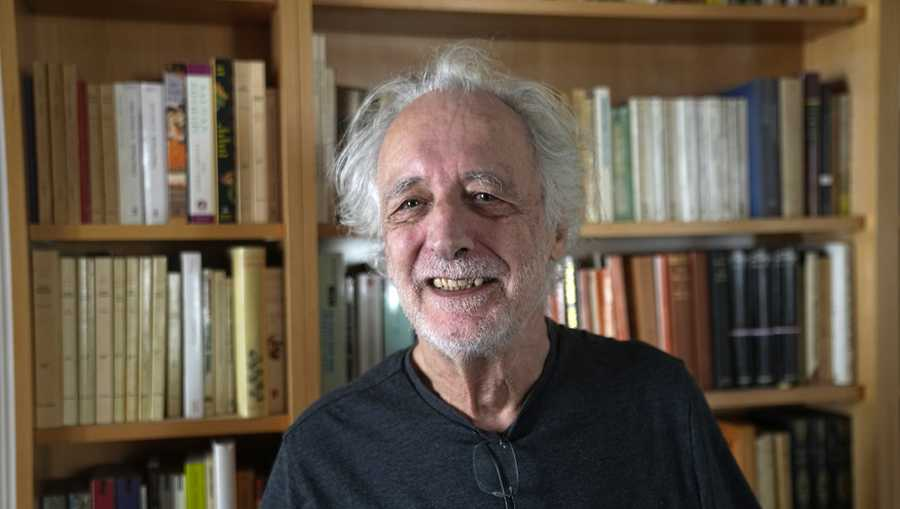
\includegraphics[width= 1\linewidth]{10}
		\caption{\small\textit{\color{timhieukhoahoc}Nhà vật lý Pháp  Pierre Agostini.}}
		\vspace*{-10pt}
	\end{figure}
	Pierre Agostini và nhóm nghiên cứu của ông tại Pháp đã thành công trong việc tạo ra và nghiên cứu một chuỗi các xung ánh sáng liên tiếp, như một đoàn tàu có nhiều toa. Họ sử dụng một kỹ thuật đặc biệt, đặt ``đoàn tàu xung" cùng với một phần bị lùi lại của xung laser ban đầu, để thấy được cách các sóng hài bậc cao đồng pha với nhau. Quá trình này cũng cho phép họ đo độ dài của các xung trong đoàn tàu, và họ nhận thấy mỗi xung chỉ dài $250$ atto giây.
	\vskip 0.1cm
	Cùng lúc đó, Ferenc Krausz và nhóm nghiên cứu của mình tại Áo đang nghiên cứu một kỹ thuật để chọn ra một xung riêng lẻ, như một toa được tách khỏi đoàn tàu và đặt sang một đường ray khác. Xung mà họ tách thành công dài $650$ atto giây và nhóm dùng nó để theo dõi và nghiên cứu một quá trình trong đó electron bị kéo ra khỏi nguyên tử.
	\vskip 0.1cm
	Những thí nghiệm này cho thấy các xung atto giây có thể được quan sát và đo, và chúng cũng có thể được sử dụng trong những thí nghiệm mới.
	\vskip 0.1cm
	Giờ thì thế giới atto giây đã mở ra, những xung ánh sáng ngắn này có thể được dùng để nghiên cứu chuyển động của electron. Hiện nay, người ta đã có thể tạo ra các xung chỉ dài vài chục atto giây, và những kỹ thuật này vẫn liên tục phát triển.
	\vskip 0.1cm
	\textbf{\color{timhieukhoahoc}Tiếp cận với chuyển động của electron}
	\vskip 0.1cm
	Các xung atto giây cho phép đo khoảng thời gian để kéo một electron khỏi nguyên tử, và xem xét sự phụ thuộc của khoảng thời gian này vào độ chặt chẽ của liên kết giữa electron với hạt nhân nguyên tử của nó. Ngày nay, có thể xây dựng lại cách mà phân bố electron dao động từ bên này sang bên kia hoặc từ nơi này đến nơi khác trong phân tử và vật chất; trước đây vị trí của chúng chỉ có thể được đo bằng một giá trị trung bình.
	\vskip 0.1cm
	Xung atto giây có thể được dùng để kiểm tra các quá trình nội tại của vật chất, và để nhận dạng các sự kiện khác nhau. Những xung này đã được dùng để tìm hiểu vật lý chi tiết của nguyên tử và phân tử, và chúng có những ứng dụng tiềm năng trong nhiều lĩnh vực, từ điện tử đến y học.
	\vskip 0.1cm
	Chẳng hạn, xung atto giây có thể được dùng để đẩy các phân tử, khiến chúng phát ra những tín hiệu đo được. Tín hiệu phát ra từ các phân tử có cấu trúc đặc biệt, một dạng ``vân tay" giúp nhận dạng phân tử, điều này có những ứng dụng tiềm năng, bao gồm chẩn đoán y tế.
\end{multicols}